\documentclass[12pt]{extarticle}

%%%%%%% PACKAGES %%%%%%%%
\usepackage[utf8]{inputenc}
\usepackage[margin=2.5cm]{geometry}
\usepackage{blindtext}
\usepackage{setspace}
\usepackage{graphics}
\usepackage{notoccite} %citation number ordering
\usepackage{lscape} %landscape table
\usepackage{caption} %add a newline in the table caption
\usepackage{hyperref}
\usepackage{enumitem}
\usepackage{datetime}
\usepackage{titlesec}
\usepackage{booktabs} % For \toprule, \midrule and \bottomrule
\usepackage{siunitx} % Formats the units and values
\usepackage{pgfplotstable} % Generates table from .csv
\usepackage{amsmath}
\usepackage{bm}
\usepackage{subcaption}
\usepackage{colortbl}
\usepackage{listings}
\usepackage{xcolor}

\definecolor{codegreen}{rgb}{0,0.6,0}
\definecolor{codegray}{rgb}{0.5,0.5,0.5}
\definecolor{codepurple}{rgb}{0.58,0,0.82}
\definecolor{backcolour}{rgb}{0.95,0.95,0.92}
\lstdefinestyle{mystyle}{
	backgroundcolor=\color{backcolour},   
	commentstyle=\color{codegreen},
	keywordstyle=\color{magenta},
	numberstyle=\tiny\color{codegray},
	stringstyle=\color{codepurple},
	basicstyle=\ttfamily\footnotesize,
	breakatwhitespace=false,         
	breaklines=true,                 
	captionpos=b,                    
	keepspaces=true,                 
	numbers=left,                    
	numbersep=5pt,                  
	showspaces=false,                
	showstringspaces=false,
	showtabs=false,                  
	tabsize=2
}
\lstset{style=mystyle}


\usepackage{chngcntr}
\counterwithin{figure}{section}
\titleformat*{\section}{\LARGE\bfseries}
\titleformat*{\subsection}{\Large\bfseries}
\titleformat*{\subsubsection}{\large\bfseries}

\newdateformat{monthyeardate}{%
	\monthname[\THEMONTH], \THEYEAR}

\onehalfspace   % 1.5 line spacing

\title{
\includegraphics[width=4cm]{pics/AAU_Logo.jpg}\\\Large{\textbf{Breast Cancer and Benign Detection using Multi-Stage Deep Convolutional Neural Networks}}
\date{}}
\begin{document}
	\clearpage\maketitle
	\begin{center}
		\vspace{-1.5cm}
		\large{\emph{Submitted by}}\\\vspace{0.5cm}
		\begin{tabular}{l l}
			
			\multicolumn{1}{p{6cm}}{ \large{\textbf{Yacoub Abu Lubad}}} &  \multicolumn{1}{p{6cm}}{\centering \large{\textbf{201930007}}} 
		\end{tabular}\\\vspace{1cm}
		\large{\emph{Supervised by}}\\\vspace{0.5cm}
		\large{\textbf{Assistant Prof. Dr. Talal A. Edwan}}\\\vspace{1cm}
		{Submitted in partial fulfillment of the requirements for the award of the Bachelor of Science in Computer Engineering Degree\\\vspace{1cm}
		Faculty of Engineering\\Al-Ahliyya Amman University\\Amman - Jordan}\\ \vspace{0.5cm}
		\Large{\textbf{\monthyeardate\today}}
		\pagenumbering{roman} % Start roman numbering
		
		\thispagestyle{empty}
	\end{center}
	\newpage
	% % Start roman numbering
	\setcounter{page}{1}
	%%% CONTENT HERE %%%%
	%j\begin{center}
	%\Large{\textbf{Acknowledgments}}\\ \vspace{1cm}
	%\end{center}
	%Acknowledgment Goes Here...
	%\newpage
	\begin{center}
		\LARGE{\textbf{Abstract}}\\ \vspace{1cm}
	\end{center}
	The implementation of Computer Vision in the prediction of breast cancer is a necessity since it cuts down a lot of costs, with the main cost in this problem is time. This graduation project documentation will discuss the different approaches towards using \emph{Artificial Intelligence (AI)} in detecting of these cancerous and non-cancerous (benign) tumors using \emph{Image Classification} and \emph{Object Detection}. The main goal is to reduce the time taken for a result to be in the reach of a professional, from weeks to matter of \textbf{seconds}. Reducing the time will not be the only goal of this graduation project, but also the need for a radiologist profession will be optional, given the circumstances of the radiologist being busy or on vacation or having a shortage of staff. This will be possible by cutting the process of waiting for a call after a screening session to only be tested again for diagnostics of the abnormality, but rather have the diagnostics appear during the screening session, cutting down the time to detect and helping out the present radiologist in highlighting the work.\\[10mm]
	Keywords: \emph{Breast Cancer\quad Classification\quad Detection}
	\newpage
	\tableofcontents
	\newpage
	\listoffigures
	\lstlistoflistings
	\listoftables
	
	\newpage
	\LARGE{\textbf{List of Abbreviations}}\\ \vspace{1cm}
	\begin{center}
		\begin{tabular}{l l}
			\multicolumn{1}{p{3cm}}{\large{\textbf{AI}}} &  \multicolumn{1}{p{8cm}}{\large{\textbf{A}rtificial \textbf{I}ntelligence}} \\
			\multicolumn{1}{p{3cm}}{\large{\textbf{ANN}}} &  \multicolumn{1}{p{8cm}}{\large{\textbf{A}rtificial \textbf{N}eural \textbf{N}etwork}} \\
			\multicolumn{1}{p{3cm}}{\large{\textbf{CNN}}} &  \multicolumn{1}{p{8cm}}{\large{\textbf{C}onvolutional \textbf{N}eural \textbf{N}etwork}}\\ 
			\multicolumn{1}{p{3cm}}{\large{\textbf{DNN}}} &  \multicolumn{1}{p{8cm}}{\large{\textbf{D}eep \textbf{N}eural \textbf{N}etwork}} \\
			\multicolumn{1}{p{3cm}}{\large{\textbf{DDSM}}} &  \multicolumn{1}{p{8cm}}{\large{\textbf{D}igital \textbf{D}atabase for \textbf{S}creening \textbf{M}ammography}} \\
			\multicolumn{1}{p{3cm}}{\large{\textbf{MS-DCNN}}} &  \multicolumn{1}{p{8cm}}{\large{\textbf{M}ulti-\textbf{S}tage \textbf{D}eep \textbf{C}onvolutional \textbf{N}eural \textbf{N}etwork}}\\ 
			\multicolumn{1}{p{3cm}}{\large{\textbf{MSOD}}} &  \multicolumn{1}{p{8cm}}{\large{\textbf{M}ulti-\textbf{S}tage \textbf{O}bject \textbf{D}etector}}\\ 
			\multicolumn{1}{p{3cm}}{\large{\textbf{MAE}}} &  \multicolumn{1}{p{8cm}}{\large{\textbf{M}ean \textbf{A}bsolute \textbf{E}rror}}\\  
			\multicolumn{1}{p{3cm}}{\large{\textbf{MLP}}} &  \multicolumn{1}{p{8cm}}{\large{\textbf{M}ulti\textbf{l}ayer \textbf{P}erceptron}}\\ 
			\multicolumn{1}{p{3cm}}{\large{\textbf{GPU}}} &  \multicolumn{1}{p{8cm}}{\large{\textbf{G}raphical \textbf{P}rpcessing \textbf{U}nit}}\\ 
			\multicolumn{1}{p{3cm}}{\large{\textbf{HDD}}} &  \multicolumn{1}{p{8cm}}{\large{\textbf{H}ard \textbf{D}isk \textbf{D}rive}}\\ 
			\multicolumn{1}{p{3cm}}{\large{\textbf{RAM}}} &  \multicolumn{1}{p{8cm}}{\large{\textbf{R}andom \textbf{A}ccess \textbf{M}emory}}
			 
		\end{tabular}
	\end{center}

	\newpage
	\LARGE{\textbf{List of Symbols}}\\ \vspace{1cm}
	\large{}
	\begin{center}
		\begin{tabular}{l l}
			{Symbol} & {Name} \\
			$b$ & bias\\
			$w$ & weights\\
			$E$ & some loss-function\\
			$\phi$ & activation function\\
			$\eta$ & cost function
		\end{tabular}
	\end{center}
	
	
	\newpage
	\large{}
	\pagenumbering{arabic}
	\section{Introduction}
	The \emph{motivation} of this graduation project will be discussed in Section \ref{Motiv}, while explaining more what the \emph{actual problem} is and the \emph{purpose of this graduation project} in Section \ref{delay problem}. As for the \emph{objectives} of this graduation project, that will be briefly discussed in Section \ref{Obj}, while the \emph{organization} and the structure of this graduation project documentation is to be discussed in Section \ref{Org}.
	\subsection{Motivation}\label{Motiv}
	
	Breast cancer is the most common cause of new cancer cases, according to the \textbf{World Health Organization (WHO)}, standing at 2.26 million recorded cases in 2020, meanwhile, the total count of cancer caused mortality cases are recorded to be 10 million in 2020, breast cancer is documented to have caused 685,000 deaths in 2020 \cite{WHO_stats}. There are multiple ways of reducing the mortality rate of this disease, one of the main approaches would be early detection. A study has proved that a delayed diagnosis and detection of \emph{more than 6 weeks} gave these cancerous cells enough time to develop into much dangerous stages, but diagnosis that were conducted \emph{under 6 weeks} of delay detected less advanced stages of these cells \cite{caplan2014delay}. So the earlier the detection of these cells are prompted, the safer and less severe it is on the patient.
	\\[5mm]
	This sort of detection is done via Screening Mammography where a patient undergoes 4 different kinds x-ray imaging, one image is taken from the side of the breast and the second is from the top, same procedure is repeated on the second breast \cite{healthline}. This totals in 4 images per patient where the radiologist can evaluate whether there are any \emph{abnormalities} detected, which are usually \emph{lumps} that are classified into two categories, \emph{Benign and Cancer}. The only downfall is that if any abnormalities are detecting after the first evaluation, the patient is contacted, which could typically take up to a week or two, to visit and perform a diagnostics test so that the abnormality could be studied even further in classifying whether it is cancerous or not \cite{healthline}.\\[5mm]
	
	\subsubsection{The result delay problem}\label{delay problem}
	As discussed in Section~\ref{Motiv}, the issues of late diagnosis and detection of these cancerous cells would increase the mortality rate, and it has also been pointed out that the results of any abnormalities detected by the radiologist could only be known after a duration of week or two. This problem can be tackled by reducing the time of detecting the abnormalities from \emph{1-2 weeks} all the way down to matter of \textbf{fractions of a second.}\\[5mm]
	This method is a great aid in early detection, this way the patient would have a time advantage to proceed to the diagnosis of this abnormality right away. However, it is also possible to \emph{skip} the diagnosis procedure as well, saving even more time when all it would require is one mammography screening and the results would be ready the moment the screening is completed.\\[5mm]
	A key feature in making this quick and accurate detection is using two methods that fall under the \textbf{Artificial Intelligence (AI)} domain, \emph{Image Classification} and \emph{Object Detection}.
	
	\subsection{Objectives}\label{Obj}
	The goal of this graduation project is to compare and contrast the different results that could be obtained using different \emph{Convolutional Neural Network (CNN)} model structures. Applying \textbf{4 different concepts} to the same dataset but with different utilization of the data to measure the accuracy that might be obtained when manipulating the data differently. Due to the vast dataset that was obtained, one of the multiple hardware constraints were during loading the images from the \emph{Hard Disk Drive (HDD)} onto the \emph{Random Access Memory (RAM)}, there was no enough memory to load the whole dataset to proceed with the model training. \\[5mm]
	A different kind of hardware constraint that was faced is the absence of \emph{Graphical Processing Unit} (GPU), a GPU is crucial for \emph{Computer Vision} (CV) due to the enormous data stream that will take place during training \cite{GPU}.
	\subsection{Organization}\label{Org}
	The \emph{Literature Review} will be discussed in \emph{Section~\ref{Lit. Rev.}} alongside the essential background on the different kinds of Neural Networks with their diverse functionalities. A deeper dive into the application's functions will be thoroughly described in \emph{Section~\ref{CV}} and the two main techniques that will be implemented in this graduation project. In \emph{Section~\ref{Meth}}, there will be a detailed explanation on the \textbf{Multi-Stage approach} that is applied to obtain the results as well as the methods that helped surpassed the constraints that were mentioned in \emph{Secion~\ref{Obj}}. Detailed dissection of the dataset will be in \emph{Section~\ref{Data}}.
	\newpage
	\section{Background}\label{Lit. Rev.}
	This graduation project will focus on implementing a \emph{Multi-Stage Object Detector}. There has been previous implementations of Brest cancer detection using a \emph{one stage} object detection, which will be explained in \emph{Section~\ref{Obj Detection}}, as seen in \cite{one_shot}, but the gap remains with setting up a \emph{two stage} object detector to detect and classify these tumors. In other words, this is an application of \textbf{Multi-Stage Deep Convolutional Neural Network (MS-DCNN)} since it relies on \emph{two stage object detection}, which will be explained in \emph{Section~\ref{Meth}}.
	\subsection{Artificial Neural Networks}\label{ANN}
	\emph{Artificial Neural Networks (ANNs)} are a simplified mathematical models that mimic the functionality of a human brain and nervous system \cite{ANN, ANN2}. Just like humans, these networks were designed to solve more complex, \emph{non-linear}, highly stochastic and multi-variable problems that a traditional program could not. These problems span out to the fields of medicine, finance, security and many more \cite{ANN_funct}. \emph{ANNs} are designed to approximating any continuous function thus are used in a wide spectrum of applications such as object detection \cite{Objdet, Objdet2}, image classification \cite{classification}, image enhancement \cite{enhancement} as well as several more uses.\\[5mm]
	The \emph{ANN} is originally compromised from multiple \emph{neurons}, or \emph{perceptron}, which can be demonstrated in \emph{Figure~\ref{fig:Perceptron}}, hence the \emph{perceptron} is the ground foundation of \emph{ANNs}.
	\begin{figure}[h]
		\centering
		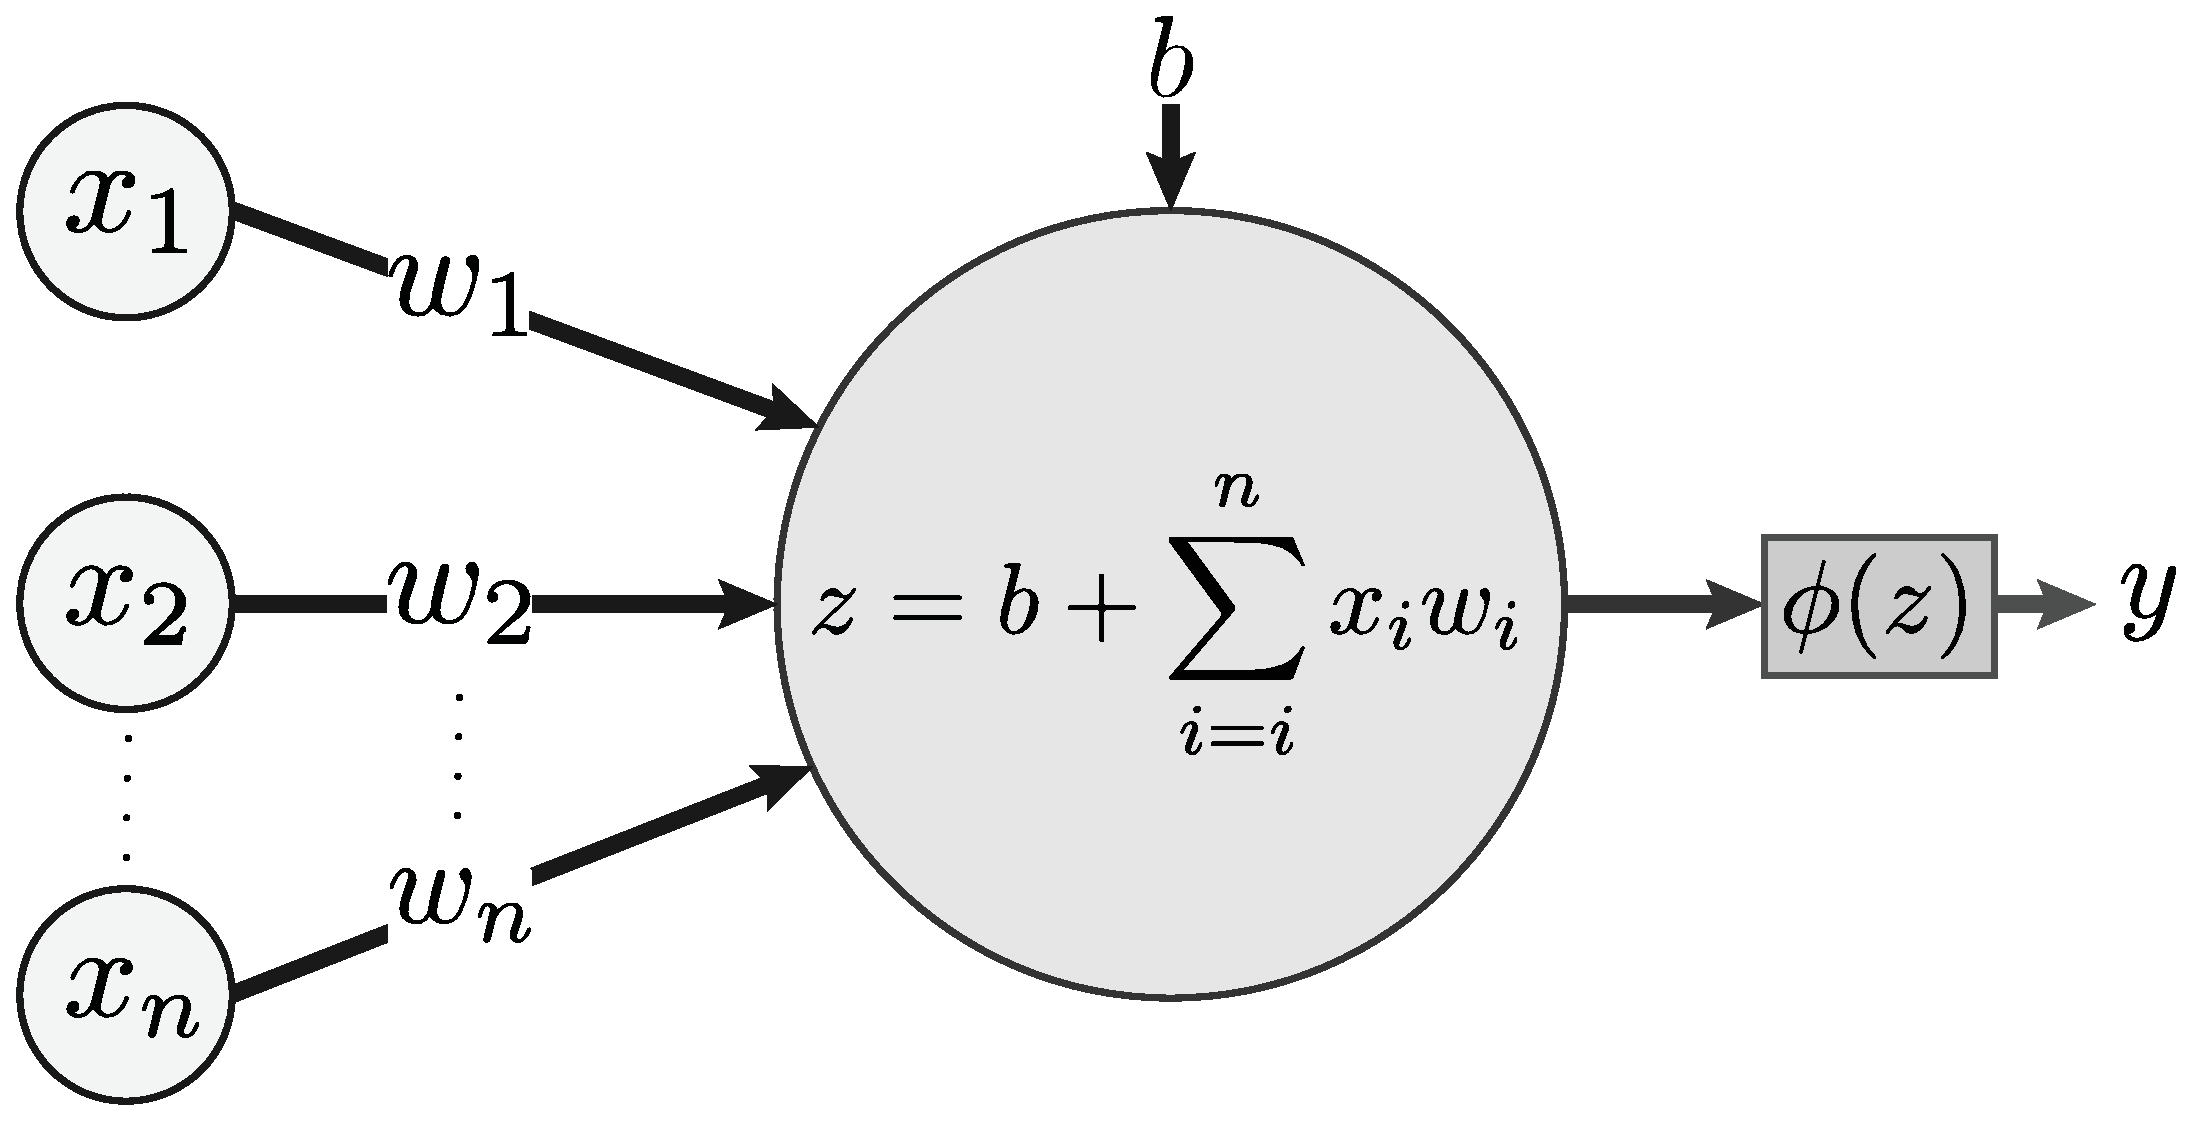
\includegraphics[width=0.7\textwidth]{pics/Figures/Perceptron.eps}
		\caption{\small{Artificial Neuron \emph{(Perceptron)}}}
		\label{fig:Perceptron}
	\end{figure}
	
	The input $\bm{x}$ of size $\bm{n}$ for this perceptron is denoted as the input vector that is composed of numerical values representing different features of a single entry as seen below.
	\begin{align}
	\bm{x} &= \begin{bmatrix}\label{inputs}
		x_1 \\
		x_2 \\
		\vdots \\
		x_n
	\end{bmatrix}
	\end{align}

	Depending on the features of a given model data, different features require different \emph{weights}, denoted as $\bm{w}$, since one feature would have more effect on the final output more than a different kind of feature, thus an input must be multiplied with a weight to determine its importance to the final output.
	\begin{align}
		\bm{w} &= \begin{bmatrix}\label{weights}
			w_1 \quad
			w_2 \quad
			\cdots \quad
			w_n
		\end{bmatrix}
	\end{align}
	
	The above vector will differ based on the next layer's size, given that there is $\bm{m}$ number of neurons in the next layer, the \emph{weight's matrix} will have a size of $\bm{m \times n}$ as seen in \emph{Equation~\ref{weights_expanded}}. The weight vector is a \emph{row vector} due to the relationship it contains with the input as every $\bm{n^{th}}$ input, there's a $\bm{n^{th}}$ weight corresponding to it.\\[5mm]
	After the input is multiplied with its assigned weight, it is now referred to as the \textbf{weighted input}, that weighted input is summed with the rest of the weighted inputs which then derives us the \textbf{weighted sum}. Then as all these inputs are summed, a \emph{bias} $\bm{b}$ is added which is an additional parameter that is used to adjust the \emph{output} of the perceptron as well as the weighted sum that is \emph{inputted} into the perceptron.\\[5mm]
	The output of the perceptron can be denoted as $\bm{y}$ and is calculated as follows:
	\begin{equation}\label{output}
		y = \phi{(z)},
	\end{equation}
	where
	\begin{equation}\label{z}
		z = b + \sum_{i}^{n} x_i w_i
	\end{equation}
	
	The $\phi$ is an arbitrary function known as the \textbf{activation function} which is responsible for causing the perceptron to \emph{fire} generating an output. This activation function is deduced by a threshold that is set based on the different types of activation functions alongside their different uses which can limit the output of reaching an undesired or unacceptable value \cite{siddique2013computational}.\\[5mm]
	One of the most common activation functions is the \emph{Rectified Linear Unit (ReLU)}\cite{agarap2018deep} which is defined as:
	\begin{equation}\label{ReLU}
		\phi(z) = max(0,z)=\Bigg\{ {z \atop 0} {\quad \atop \quad} {z \atop z} {> \atop <} {0 \atop 0}
	\end{equation}
	and it is widely used in \emph{Neural Networks} as the \emph{hidden layer's} perceptrons', which is discussed in \emph{Section~\ref{MLP}}, activation function. 
	\\[5mm]
	The expansion from a single perceptron to multi perceptrons forms a \emph{single layered neural network} as seen in \emph{Figure~\ref{fig:ANN}}; using the input vector as seen in \emph{Equation \ref{inputs}} and defining the weights matrix 
	\begin{align}
		 W &= \begin{bmatrix}\label{weights_expanded}
			w_{1,1}\quad w_{1,2} \quad \cdots \quad w_{1,n}\\
			w_{2,1} \quad w_{2,2} \quad \cdots \quad w_{2,n}\\
			\vdots \qquad \vdots \qquad \ddots \qquad \vdots\\
			w_{m,1} \quad w_{m,2} \quad \cdots \quad w_{m,n}
		\end{bmatrix}
	\end{align}
	where $\bm{m}$ is the number of perceptrons and $\bm{n}$ is the number of inputs. The weight responsible for the $\bm{n^{th}}$ input and $\bm{m^{th}}$ perceptron is written as $\bm{w_{m,n}}$. While the bias vector is defined as:
	\begin{align}
		\bm{b} &= \begin{bmatrix}\label{bias_vector}
			b_1 \\
			b_2 \\
			\vdots \\
			b_m
		\end{bmatrix}
	\end{align}

	\begin{figure}[h]
	\centering
	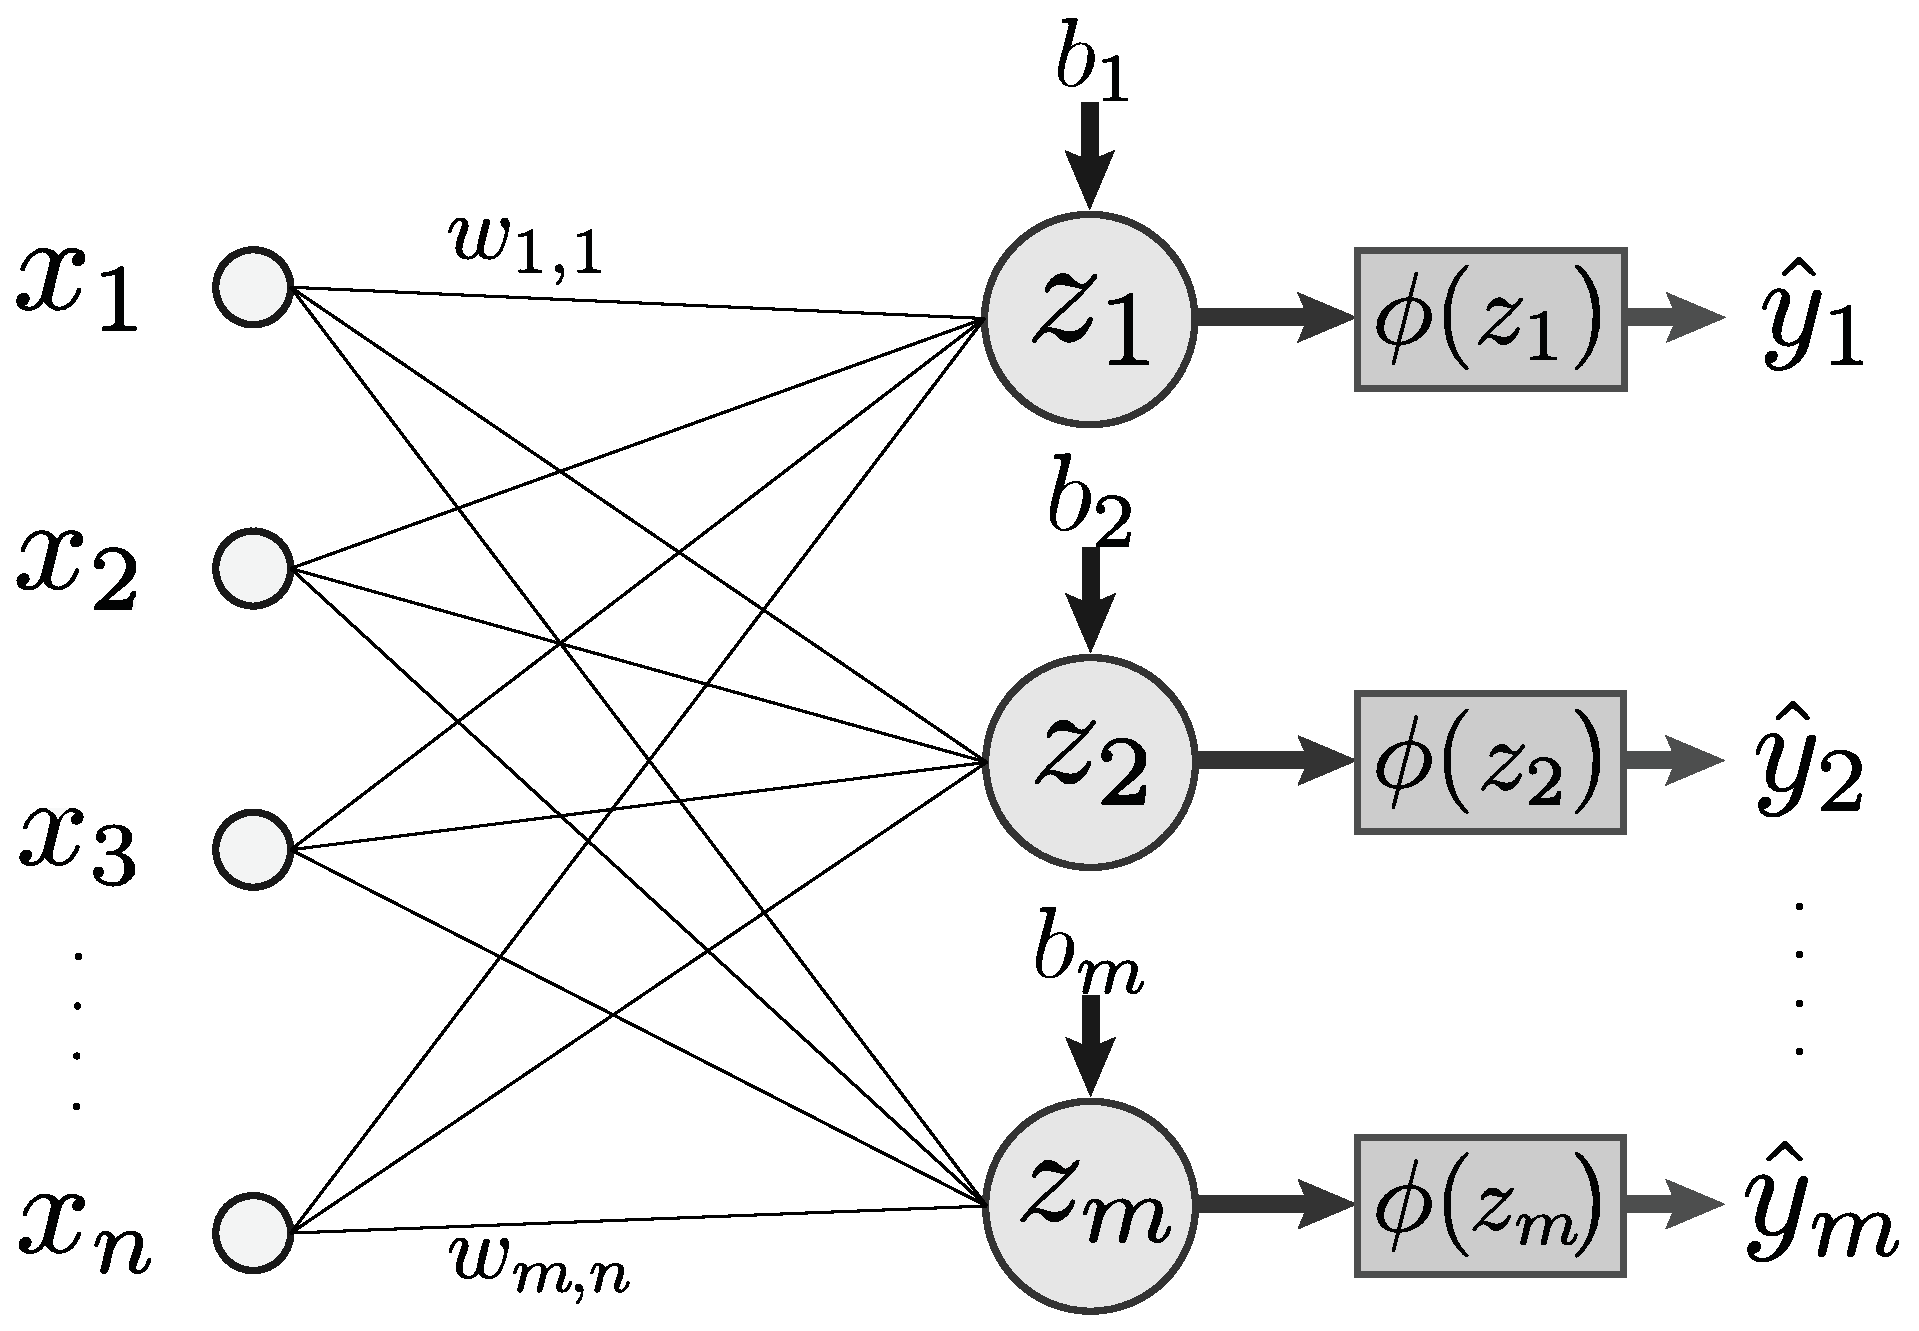
\includegraphics[width=0.7\textwidth]{pics/Figures/ANN.eps}
	\caption{\small{Artificial Neural Network Model \emph{(Single Layer)}}}
	\label{fig:ANN}
	\end{figure}

	The \emph{multi-perceptron, single layer, output} can be computed as:
	\begin{equation}\label{y_hat}
		\bm{\hat{y}} = \phi(\bm{b}+ W\bm{x})
	\end{equation}
	So far, this has been a \textbf{feed-forward} neural network without any kind of \emph{learning}, for the network to start learning there must be a \emph{weight update} algorithm which updates the weights regularly after every entry. This algorithm is known as \emph{Backpropagation} \cite{backprop}, and the formula can be seen in \emph{Equation \ref{backprop}} below: 
	\begin{equation}\label{backprop}
		W^{t+1} = W^{t} - \eta\dfrac{E}{\Delta{W}}
	\end{equation}
	where $W^{t}$ denotes the weight at iteration $t$ of the gradient descent and $\eta$ is a \emph{cost function}.\\[5mm]
	\textbf{Cost functions}, also technically known as \textbf{Loss functions}, vary depending on the faced problem and the desired output of the neural network, for instance, a \emph{Regression} problem will most likely use a \textbf{Mean Absolute Error (MAE)}\cite{qi2020mean} as a cost function which can be computed as:
	\begin{equation}\label{MAE}
		MAE = \dfrac{\sum_{1}^{n}|y_i-x_i|}{n}
	\end{equation}
	where $y_i$ is the predicted value, $x_i$ being the true value and $n$ the total number of data points. However, an \emph{Image Classification} problem will most likely use \textbf{Categorical Crossentropy}\cite{ho2019real} which quantifies the difference between probability distributions in a a multi-class classification problem and it can be computed as:
	\begin{equation}\label{crossentro}
		E = \dfrac{-(\sum_{1}^{N}y_i\log(x_i))}{N}
	\end{equation}
	where $y_i$ is the predicted value, $x_i$ being the true value and $N$ the number of classes.

	
	\subsubsection{Multilayer Perceptrons}\label{MLP}
	\emph{Multilayer Perceptrons (MLPs)} is one class of the \emph{feed-forward ANNs} where, at least, one \textbf{hidden layer} is present between the input layer and the output layer, a demonstrative diagram can be seen in \emph{Figure~\ref{fig:MLP}}, the hidden layers act like a \emph{black box} where the objective of this so called black box is to extract features from the input, the \emph{deeper} the network, the more features it will be able to extract. But having a \emph{Deep Neural Network (DNN)} could be troubling sometimes as there would be more than 2-3 layers which, in coherence to the more feature extraction, it also acts in a much more complex way which applies a lot of constraints in areas such as software and hardware. The reason for the software constraint with \emph{DNN} is that it will require more data to learn unlike shallower models. As for hardware constraints, the process that is responsible for training \emph{DNNs} is known as \emph{Deep Learning}, Deep Learning requires advanced \emph{GPUs} which could get costly for a user, the essence of a GPU is crucial due to the time constraint that might be present in the absence of a GPU \cite{GPU}. \\[5mm]
	The \emph{black box} could be seen also in \emph{Figure~\ref{fig:MLP}} as a light gray box captioned \emph{Hidden Layers}. 
	
	\begin{figure}[h]
		\centering
		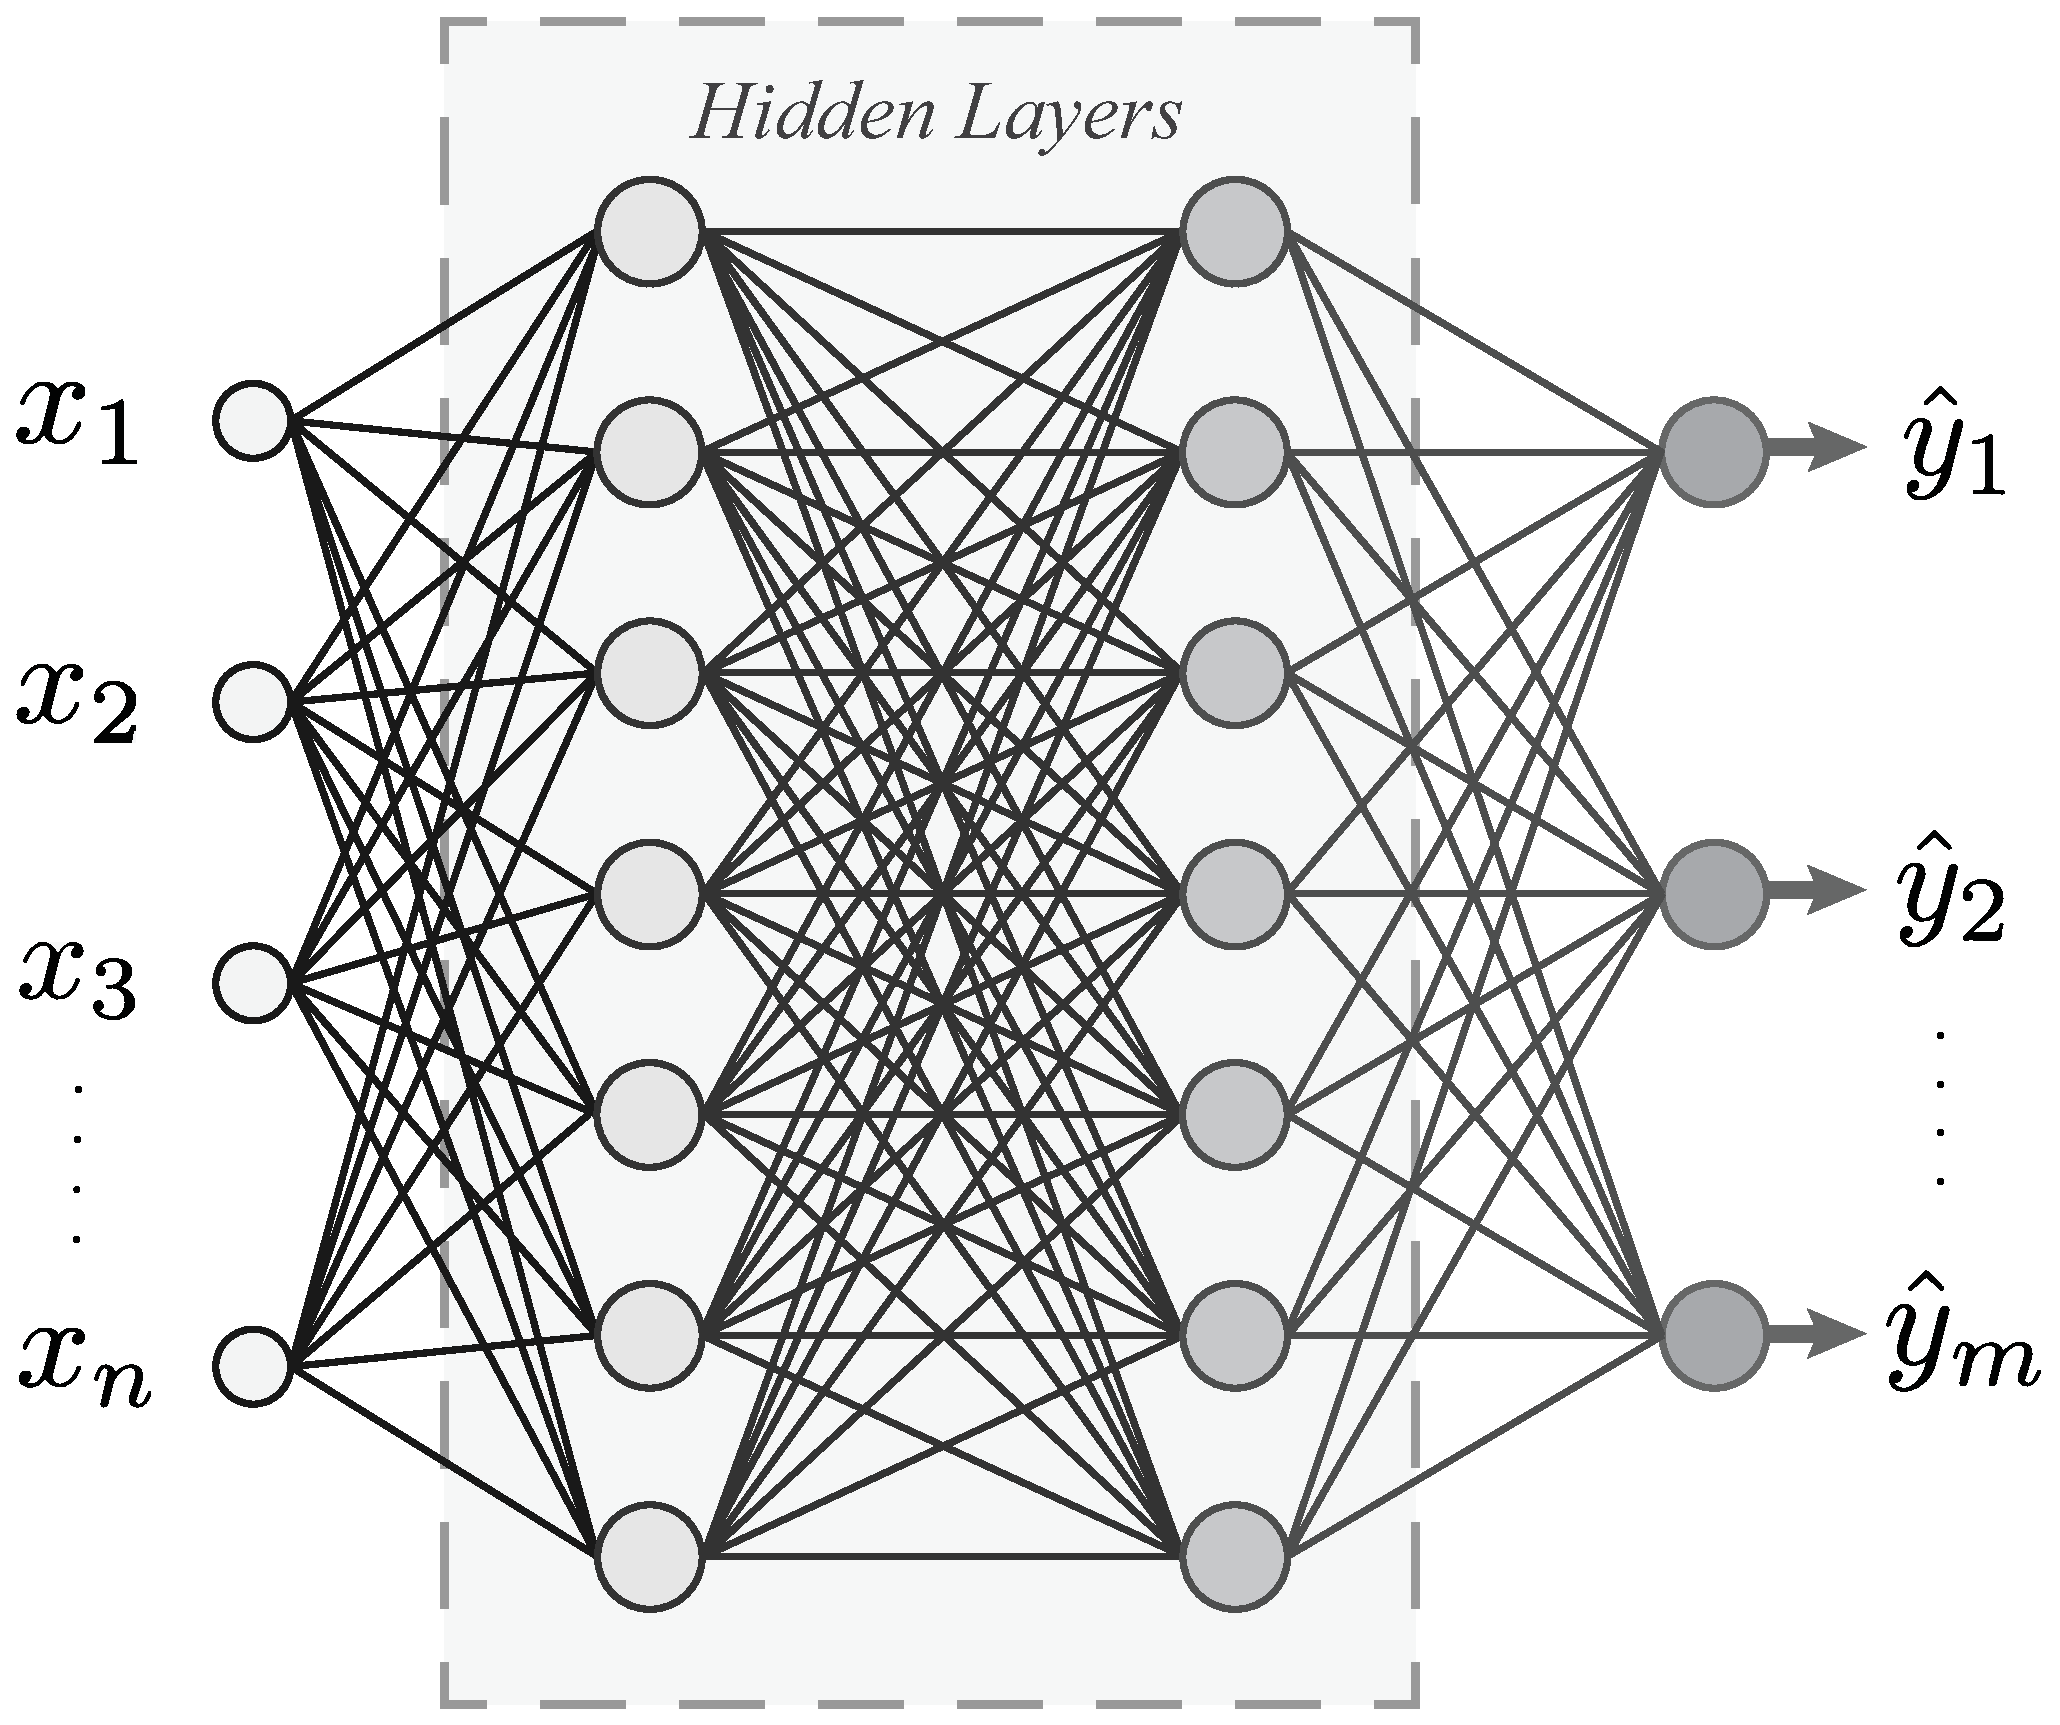
\includegraphics[width=0.7\textwidth]{pics/Figures/MLP.eps}
		\caption{\small{Three layer feed-forward network}}
		\label{fig:MLP}
	\end{figure}
	
	However, each layer, of these hidden layers, is still computed as \emph{Equation~\ref{y_hat}}. Bare in mind that the input of the next layer would be the previous layer's computed $\bm{\hat{y}}$, using \emph{Equation~\ref{y_hat}} for the first layer and computing the output layer number $\bm{i}$ as:
	\begin{equation}\label{ANN_y_hat}
		^{(i)}\bm{\hat{y}} = \hspace{1mm} ^{(i)}\phi(^{(i)}\bm{b}+ ^{(i)}W^{(i-1)}\bm{\hat{y}})
	\end{equation}
	\emph{where $\bm{i \geq 2}$}\\
	Moreover, layers where each perceptron is connected to every perceptron of the following layer, as seen in \emph{Figure~\ref{fig:MLP}}, are called \emph{dense} or \emph{fully connected} (FC) layers.
	
	\subsubsection{Convolutional Neural Networks}\label{CNN}	
	\emph{Section~\ref{MLP}} included an explanation on \emph{ANNs} and how it helps in learning more complex functions using deeper networks, however image inputs are not suitable for \emph{MLPs}, since \emph{MLP} networks handle vector inputs, hence requiring the image to be flattened leading to an extreme increase in number of trainable parameters. In other words, using an image of size (512x512) as an input to extract the features would lead to a single perceptron containing \textbf{262.144} trainable parameters (excluding bias) and increasing number of perceptrons in the first hidden layer to around 100, which is not convenient for the size of the image but just setting it as an example, would set the number of trainable parameters to an astonishing \textbf{26.214.400} just for the first layer. In addition, increasing the resolution of the image and using a three-channel \emph{RGB} image will also exceedingly increase the trainable parameters. Therefore, a different kind of architecture is needed to handle images, and that new architecture is called \emph{Convolutional Neural Network (CNN)}.\\[5mm]
	As stated in \cite{DL}, ”Convolutional networks are simply neural networks that use convolution in place of general matrix multiplication in at least one of their layers”. For an input image $I$ and kernel (filter) $K$ , the discrete convolution operation is defined as \cite{DL}:

	\begin{equation}\label{conv}
		c_{i,j} = (I*K)_{i,j} = \sum_{m}\sum_{n}I_{m,n}K_{i-m,j-n}
	\end{equation}
	In general the convolution operation on these images would produce an output feature image which is produced by convolving the input image with the kernel, the kernel would be a set of weights (trainable parameters) which the size could be defined by a user.\\[5mm]
	Although many implementations talk about convolution and applying \emph{Equation~\ref{conv}} to the "\emph{Convolutional} Neural Network", an alternative method is used which is called \emph{cross-correlation}. As we can see in \emph{Equation~\ref{conv}}, where $m$ and $n$ iterate over valid subscripts of both $I_{m,n}$ and $K_{i-m,j-n}$, the \emph{filter} $K$ is flipped thus producing a \textbf{flipped} output, since the filter would be sliding in the negative direction. Consequently, an alternative variant is introduced called \emph{cross-correlation} and it is computed as follows:
	\begin{equation}\label{cross-corr}
		c_{i,j} = (I*K)_{i,j} = \sum_{m}\sum_{n}I_{i+m,j+n}K_{i,j}
	\end{equation}
	Hence producing an output which is not flipped as seen in \emph{Figure~\ref{fig:cross-corr}}. 
	
	\begin{figure}[h]
		\centering
		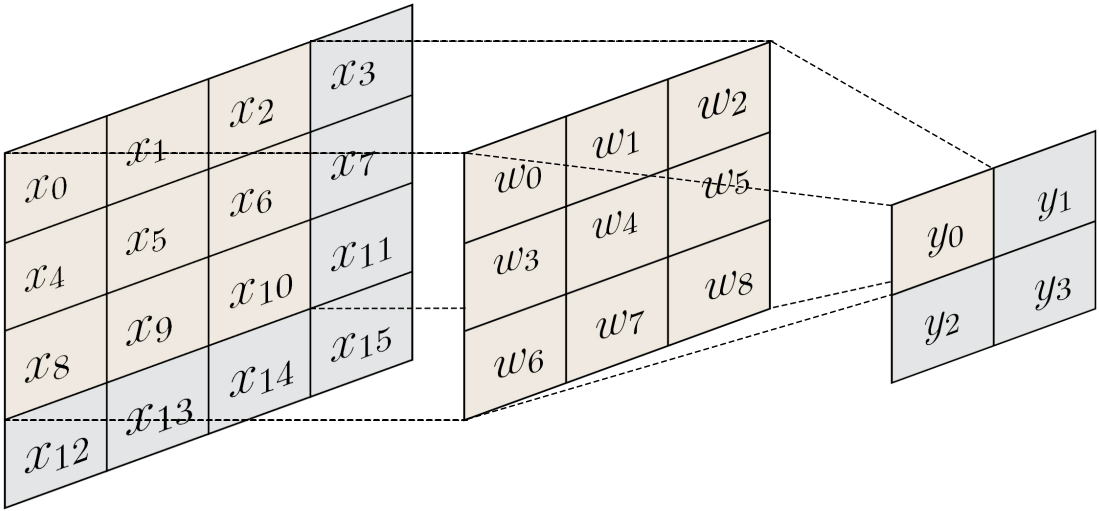
\includegraphics[width=0.8\textwidth]{pics/Figures/convolution.png}
		\caption{\small{An illustration of \emph{Cross-Correlation}}}
		\label{fig:cross-corr}
	\end{figure}
	The process can be seen as the summation of the element-wise product between the kernel and any spatial location of center $(i, j)$, then moving the kernel by the amount of \emph{stride }to another location until the whole image is covered. Additionally, for multi-channel input image the \emph{Equation~\ref{cross-corr}} can be expanded as follows:
	\begin{equation}
		c_{i,j} = (I*K)_{i,j} = \sum_{m}\sum_{n}\sum{d}I_{i+m,j+n,d}K_{i,j,d}
	\end{equation}
	where d iterates over valid subscripts of both $I_{i+m,j+n,d}$ and $K_{i,j,d}$. Note it is frequent to add bias to the equation. Multiple kernels can be applied to the same input image to obtain several feature maps. Thus, the output depth is equal to number of kernels / filters applied. One of the characteristics of a convolutional layer is \textbf{parameter sharing}; it is possible to assume that if a specific filter is useful in some region, then it is useful in other regions as well. Under this assumption, the parameters are shared along the depth \cite{par_share} reducing the number of learnable parameters. Moreover, it is frequent to apply an activation function to feature maps in order to obtain activation maps.
	\\[5mm]
	Convolution reduces the size of the input image. For this reason, when several convolution layers are used, the image size decreases drastically. As a counter-measurement, an outer frame is added to the image, limiting the size reduction. This process is called \textbf{padding}. It is common to use zeros as values for the frame and this is called \emph{zero padding}, while reflecting values of rows and columns into the frame is named \emph{reflection padding}.\\[5mm]
	For an image of height $(H_i)$ and width $(W_i)$, the size of the image post convolution is computed as:
	\begin{equation}\label{width}
		\hat{W}_i = \dfrac{W_i-k+2P_i}{s}+1
	\end{equation}
	\begin{equation}\label{height}
		\hat{H}_i = \dfrac{H_i-k+2P_i}{s}+1
	\end{equation}

	where $\hat{W}_i$ and $\hat{H}_i$ are the new width and height, respectively, of post convolution process. $k$ is the kernel size, $s$ being the stride and the padding size denoted as $P_i$. 
	
	\begin{figure}[h]
		\centering
		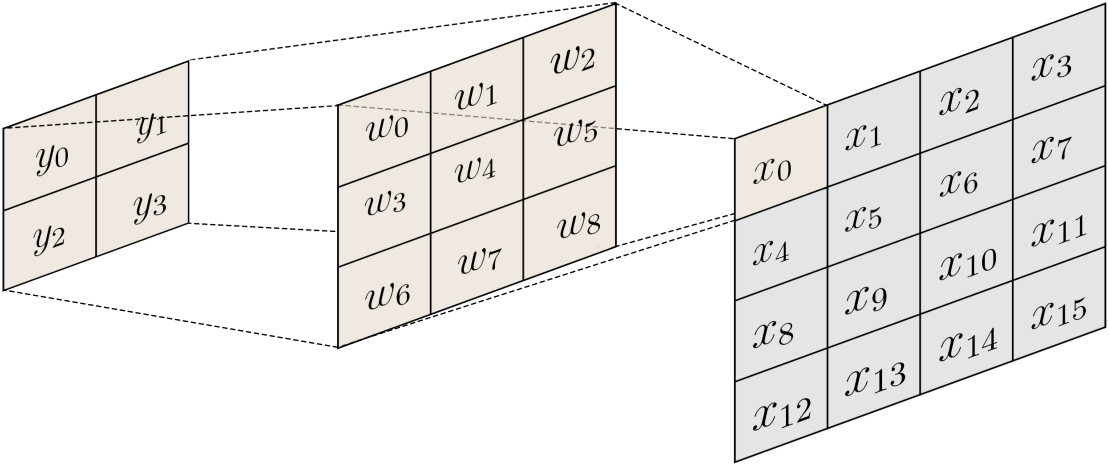
\includegraphics[width=0.8\textwidth]{pics/Figures/reverse_convolution.png}
		\caption{\small{An illustration of \emph{Transposed Convolution}}}
		\label{fig:T_Conv}
	\end{figure}
	
	In a convolutional layer, the kernel defines a convolution that has a forward pass and backward pass. Flipping the passes would result in \emph{Transposed Convolution} or known as \emph{fractionally strided convolution} \cite{stride}, which is used for upsampling. Transposed Convolution can as well be visualized in \emph{Figure~\ref{fig:T_Conv}}.
	\subsection{Computer Vision}\label{CV}
	\emph{Human vision} is similar to \emph{Computer Vision (CV)}, with the exception that people have a head start. Human vision benefits from lifetimes of context to teach it how to distinguish objects apart, how far away they are, whether they are moving, and whether something is incorrect with an image. CV teaches computers to execute similar tasks, but using cameras, data, and algorithms rather than retinas, optic nerves, and a visual cortex, it must do it in a \textbf{fraction of the time}. Because a system trained to check items or monitor a production asset can assess hundreds of products or processes per minute, detecting faults or issues that are invisible to humans, it can swiftly \textbf{outperform humans}. The speed and the methods will be discussed in \emph{Section~\ref{Classification}} and \emph{Section~\ref{Obj Detection}}.
	\subsubsection{Image Classification}\label{Classification}
	\emph{Image Classification} tasks are generally easy to grasp, it is simply the discrimination between classes, whether \emph{Binary} or \emph{Multi-Class} classification, a classifier's task will be to pick up on the features of each class and \emph{learn} them to be able to label input data. Binary Classification and Multi-Class Classification is displayed clearly in \emph{Figure~\ref{fig:class}}.
	\begin{figure}
		\centering
		\subfloat[\centering Binary Classification \cite{TensorFlow_PL}]{{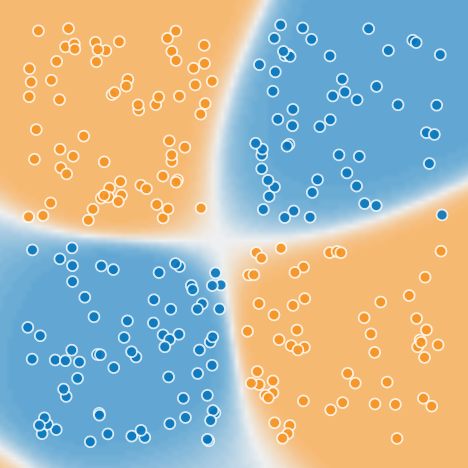
\includegraphics[width=6cm]{pics/Figures/Classification.png} }}%
		\qquad
		\subfloat[\centering Multi-Class Classification \cite{Multi_class}]{{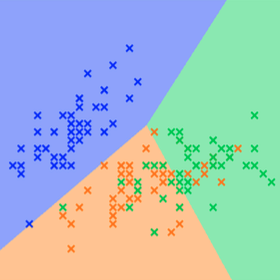
\includegraphics[width=6cm]{pics/Figures/Multi_Class.png} }}%
		\caption{Displaying the difference between binary and multi-class classification}
		\label{fig:class}
	\end{figure}
	Knowing that a classifier can classify multiple classes and not necessarily just a binary classification, this also means that it can classify up to $\bm{n}$ numbers of classes. A good example of multi-class classification is the MNIST hand-written digit classification \cite{mnist}, this problem hosts \textbf{60.000} hand-written \textbf{labeled} digits, as seen in \emph{Figure~\ref{fig:MNIST_img}}, where $\bm{n = 10}$ as we have 10 numerical digits. 
	\begin{figure}[h]
		\centering
		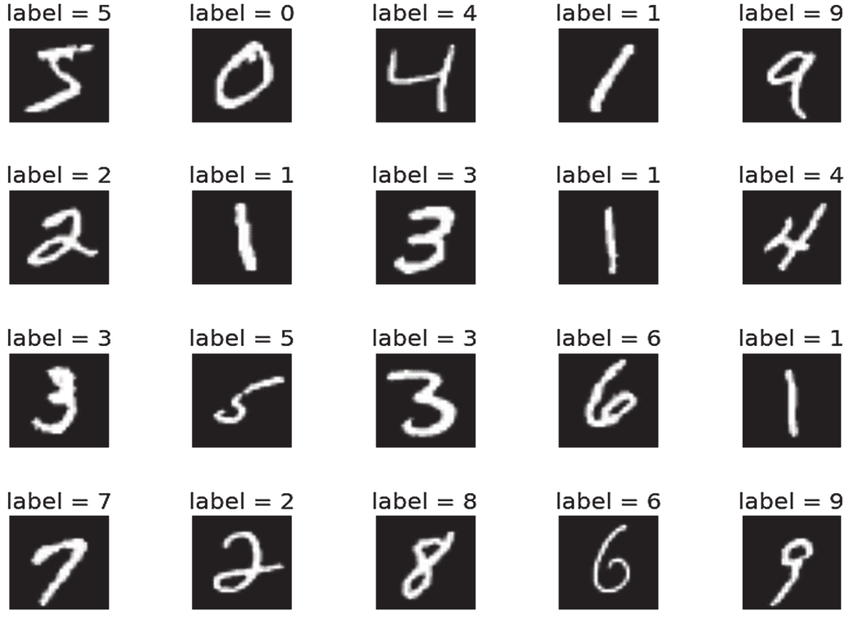
\includegraphics[width=0.7\textwidth]{pics/Figures/mnist.png}
		\caption{\small{MNIST dataset with each class represented above the image respectively}}
		\label{fig:MNIST_img}
	\end{figure}
	This sort of dataset is fed into an Image Classifier which then develops an understanding of the differences each hand-written digit contains, this classifier then outputs the estimated label of the digit. A classifiers flow is seen in in \emph{Figure~\ref{fig:Classifier}}.
	\begin{figure}[h]
		\centering
		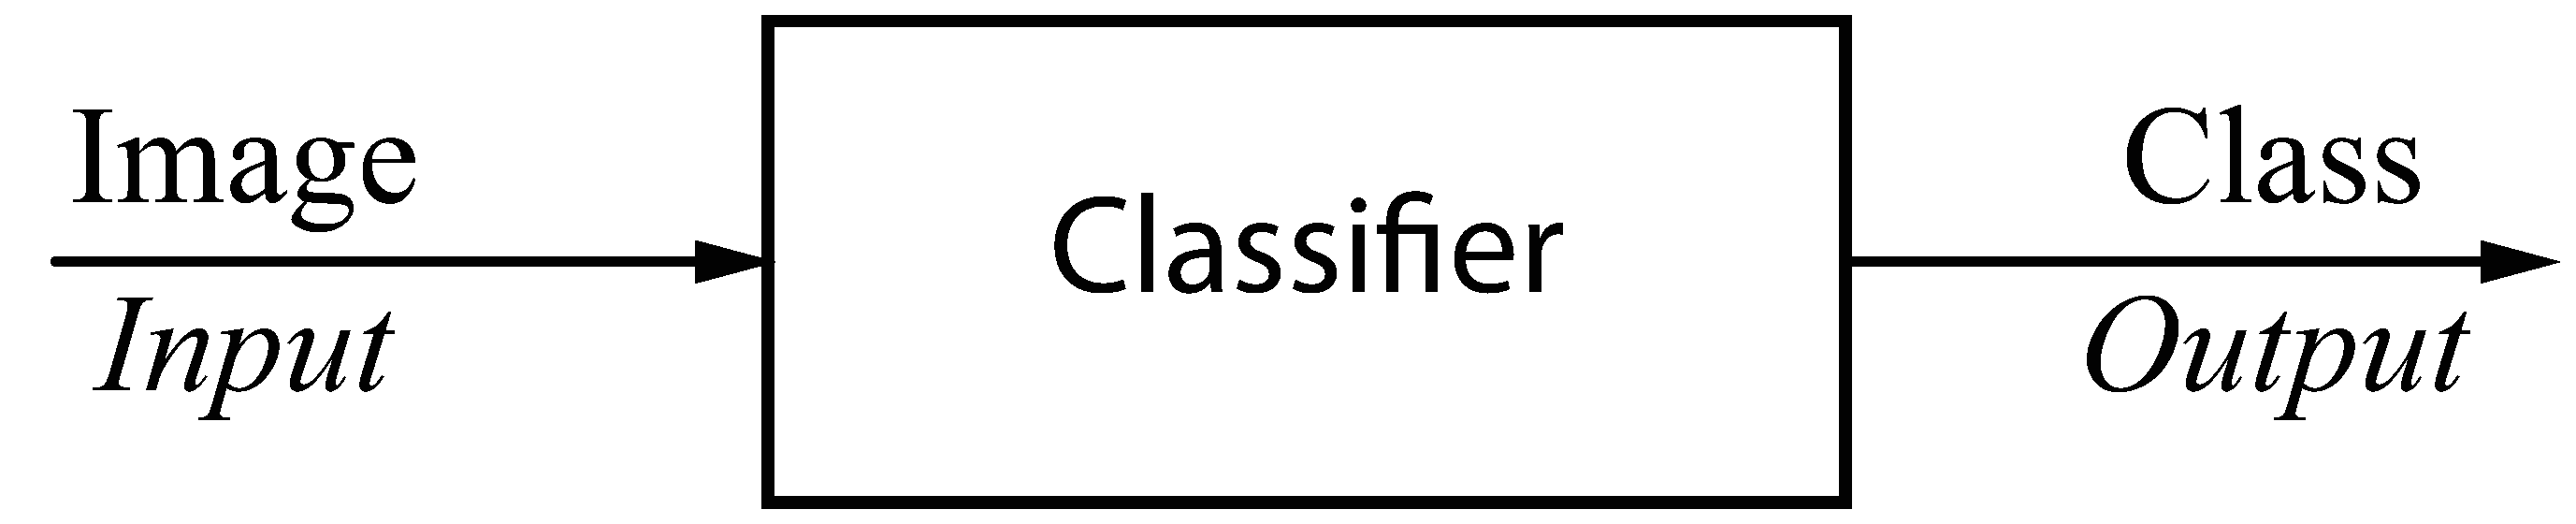
\includegraphics[width=0.5\textwidth]{pics/Figures/Classifier_Block_Diagram.eps}
		\caption{\small{Classifier Diagram}}
		\label{fig:Classifier}
	\end{figure}
	\subsubsection{Object Detection}\label{Obj Detection}
	In an object detection task, a model has to both classify objects / instances appearing in an image and localize them within the image. The localization is represented by a 2D bounding box, in which the structure of the object detector is visible in \emph{Figure~\ref{fig:Obj Detector}}. State of the art networks tackling this task are divided into two main groups. The first group are the single stage object detection network, which prioritize the \textbf{inference speed} over than the accuracy. Single stage methods include \emph{YOLO} \cite{Objdet2} and \emph{RetinaNet} \cite{Retina}.The second group of methods is the two stage methods, which are tuned for \textbf{accuracy} over inference speed. An example of two stage methods is the Faster R-CNN \cite{Objdet}.
	\begin{figure}[h]
		\centering
		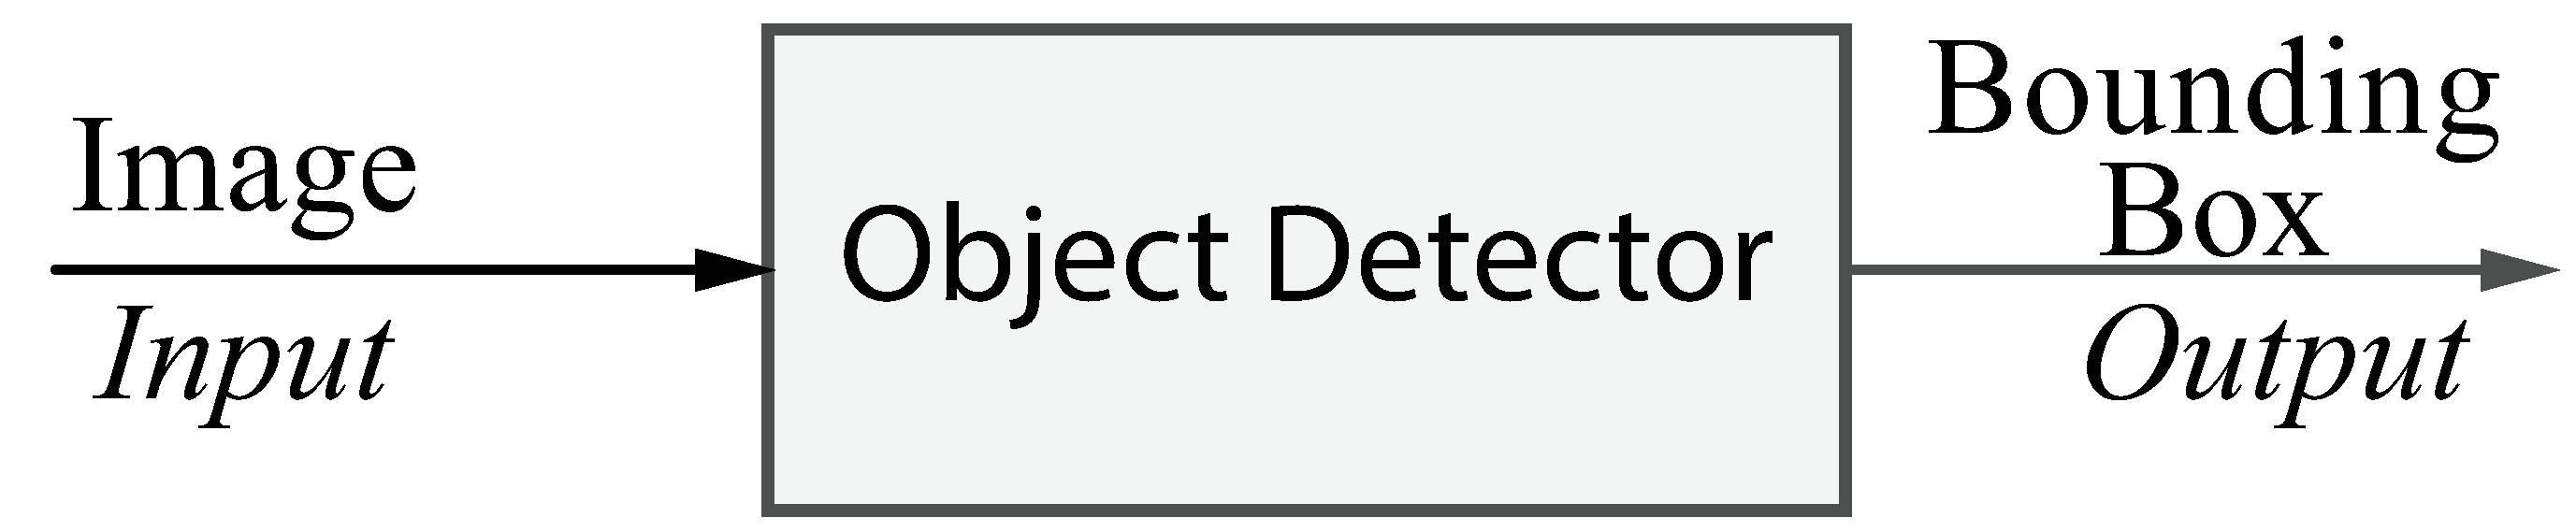
\includegraphics[width=0.5\textwidth]{pics/Figures/Obj_Det_Block_Diagram.eps}
		\caption{\small{Object Detection Diagram}}
		\label{fig:Obj Detector}
	\end{figure}
	Unlike Image Classification, Object Detection is only responsible for detecting and localizing learned features no matter how many \emph{Classes'} features a detector learns. In instance when it comes to the two different kinds of object detectors, single and two stage detectors, this graduation project will conduct the two stage object detector method as the results do not really rely on inference speed. And as discussed earlier, single stage object detectors would prioritize inference speed over accuracy as they would be widely used in real-time object detection. However, the dataset, which will be discussed in \emph{Section~\ref{Data}}, is not a live image but rather a static image which is processed after performing x-ray imaging \cite{mammography}. An object detector learns by inputting a single object that is restrained by a bounding box or a mask. An image with a contour mask could be seen in \emph{Figure~\ref{fig:img_cont}}.
	\begin{figure}
		\centering
		\subfloat[\centering Image containing cancer cell]{{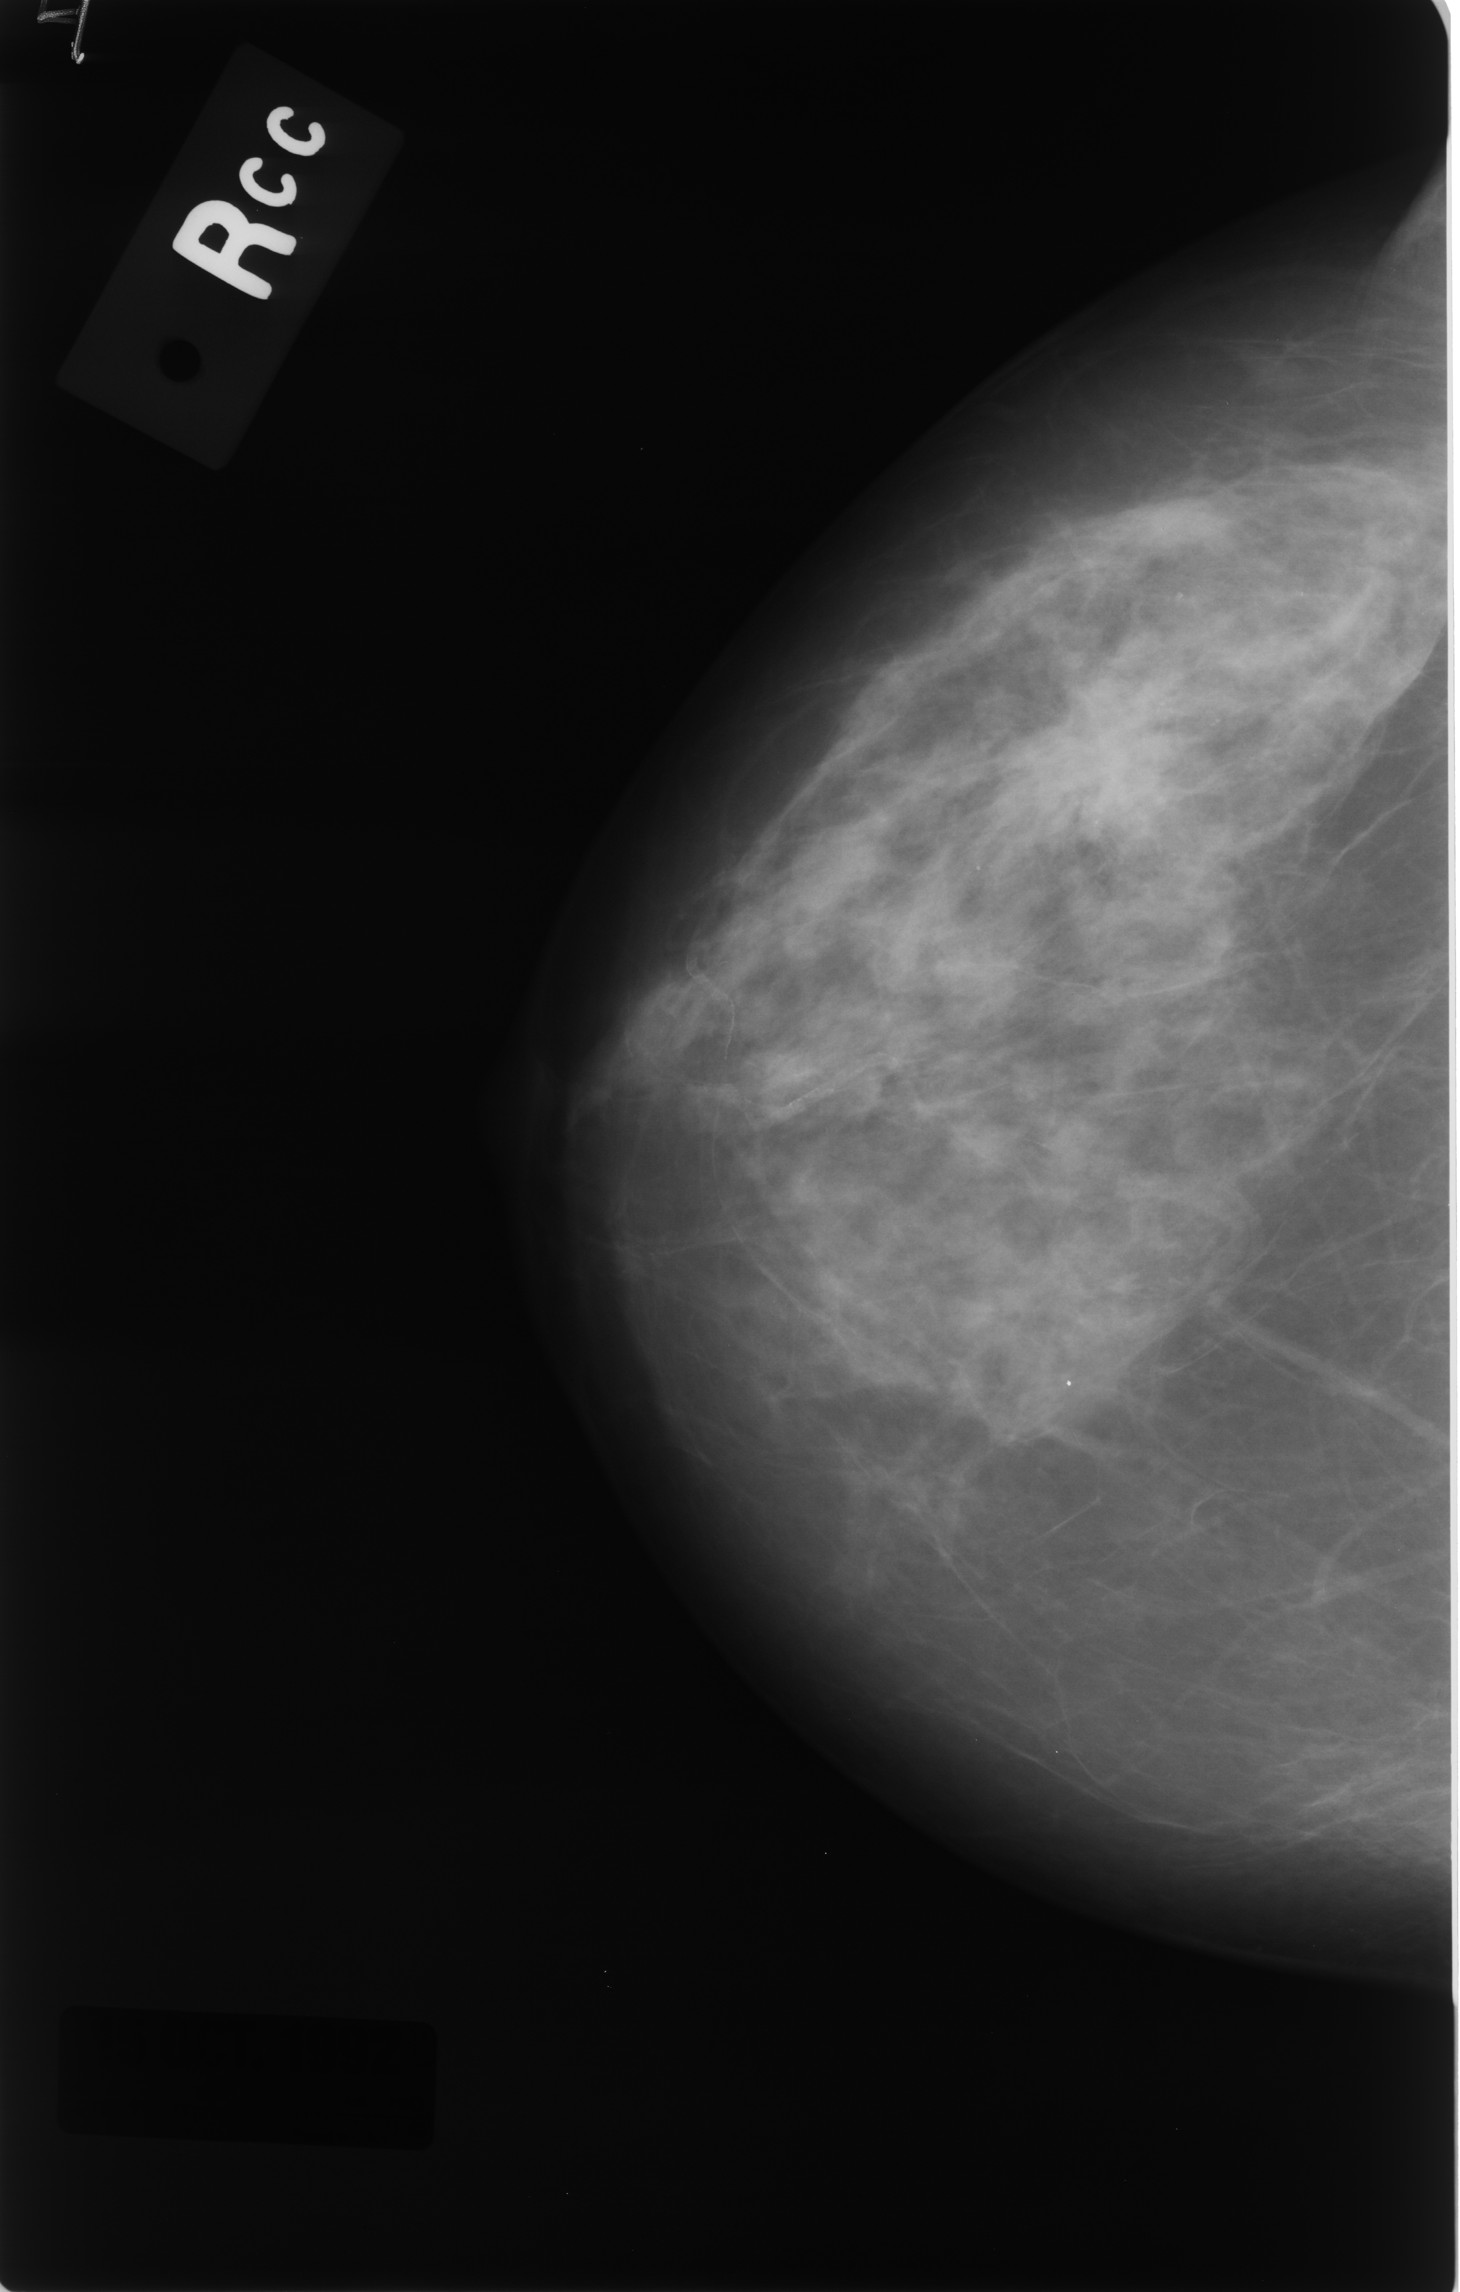
\includegraphics[width=4.5cm]{pics/Figures/cancer_img.jpg} }}%
		\qquad
		\subfloat[\centering Contour Mask]{{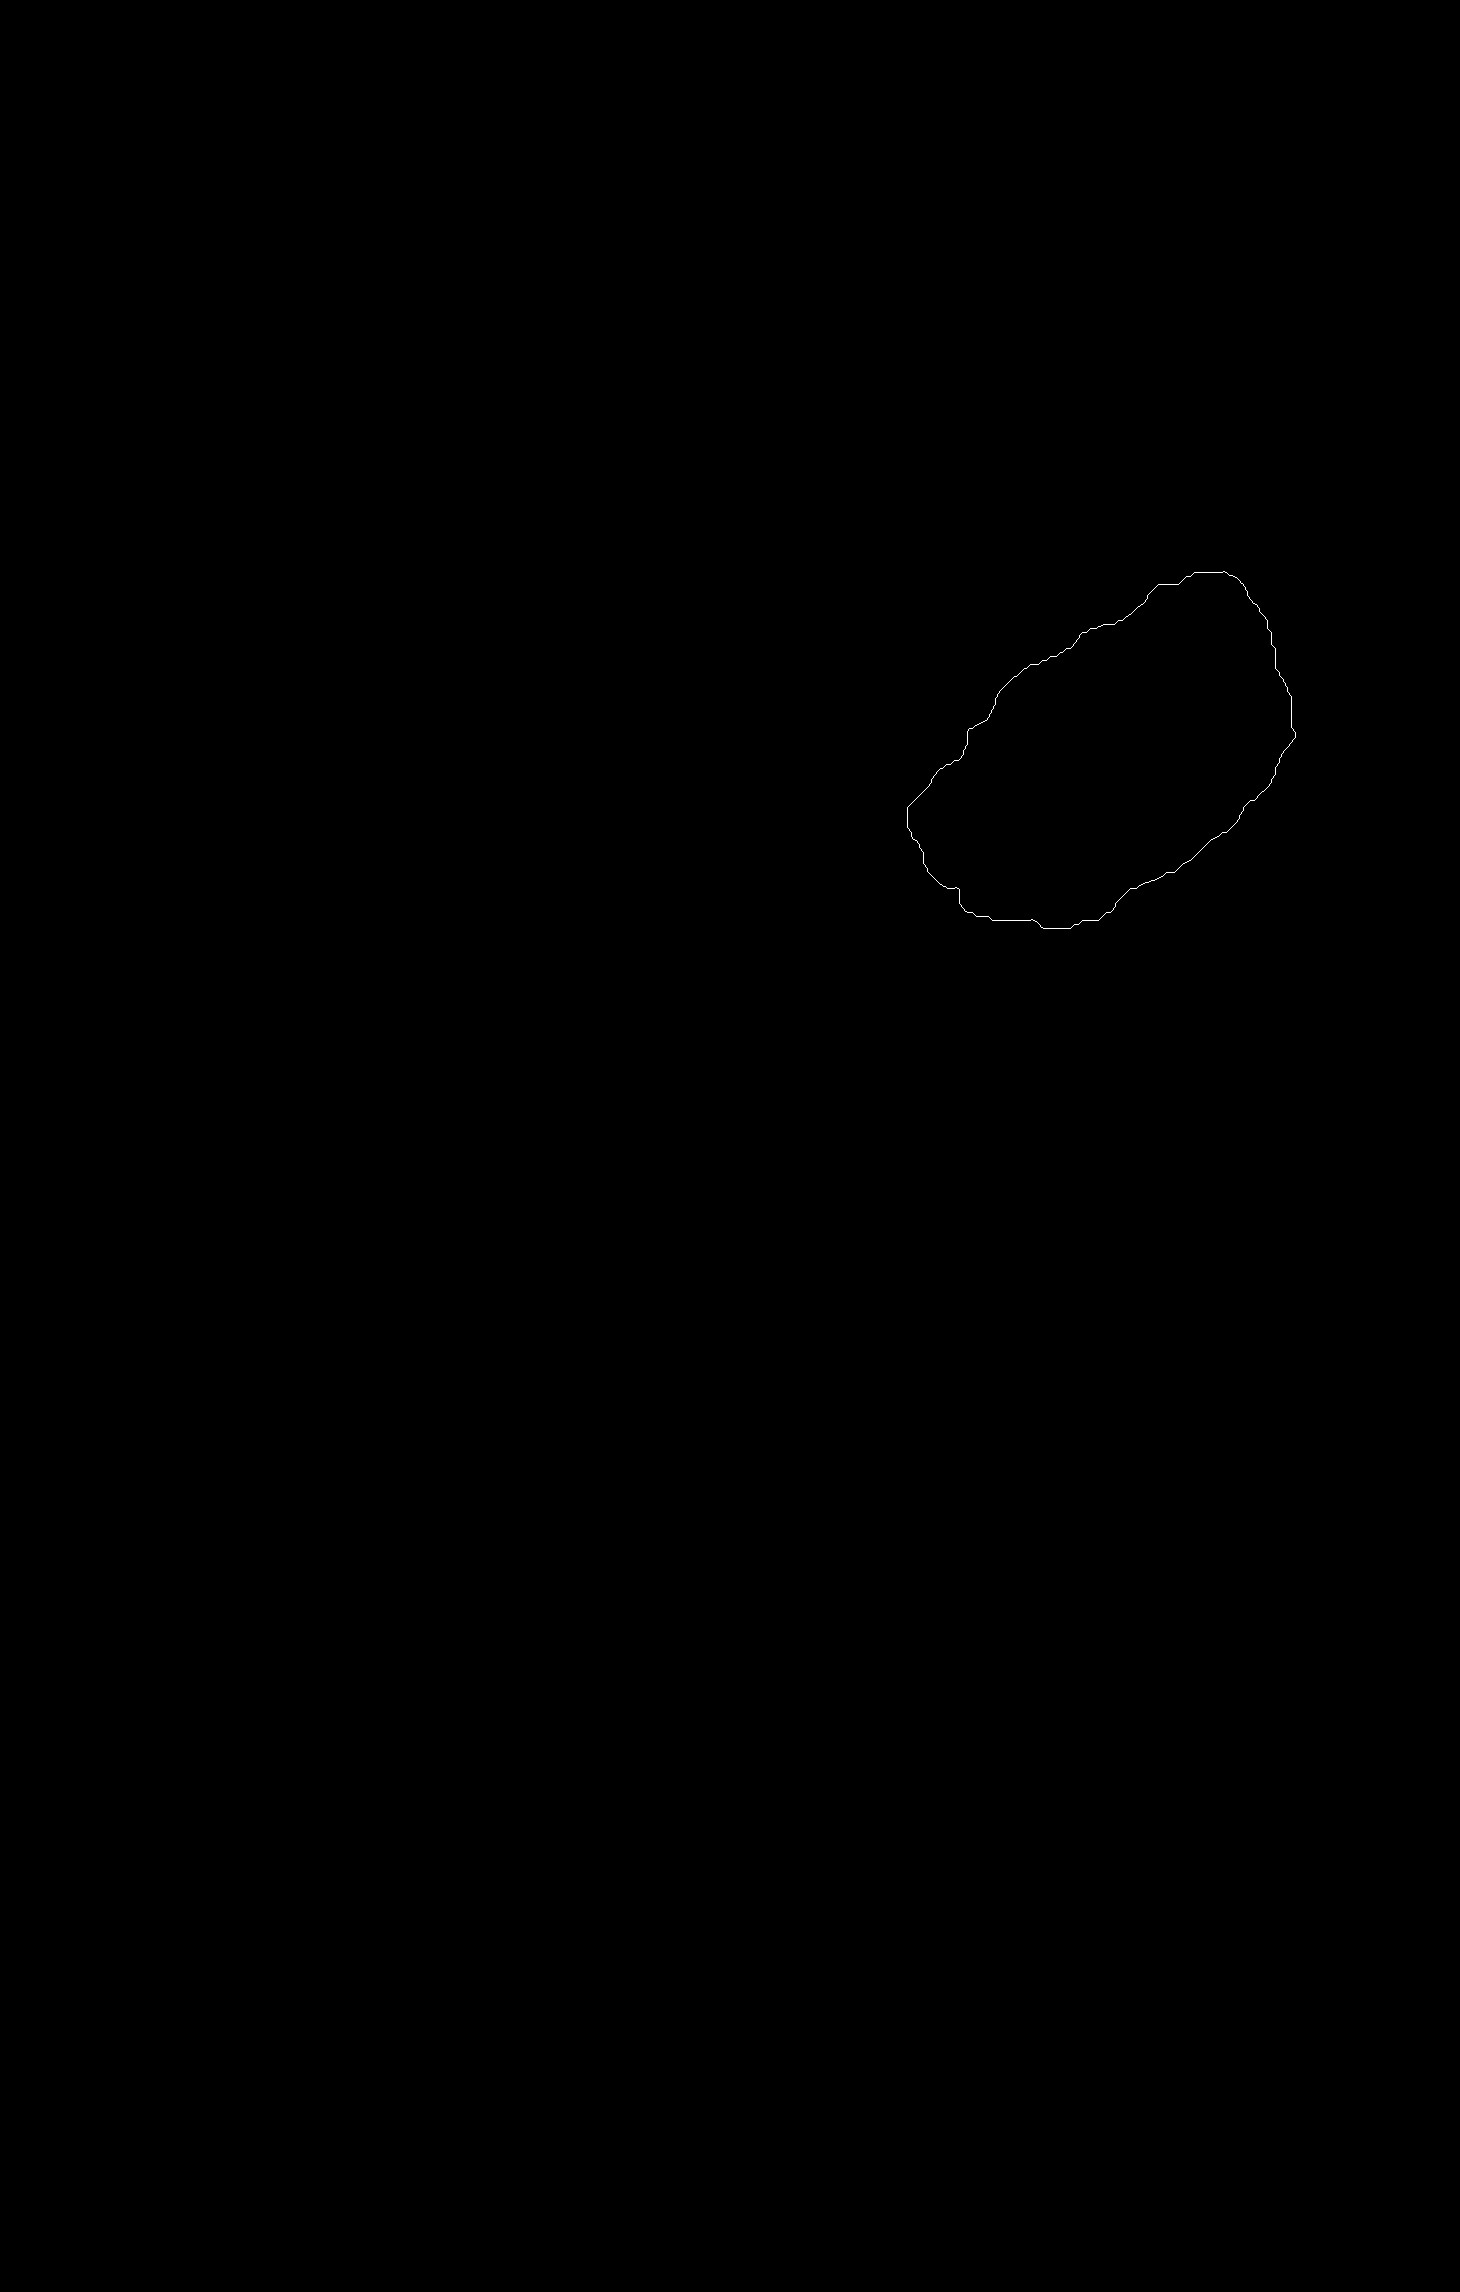
\includegraphics[width=4.5cm]{pics/Figures/contour_img.jpg} }}%
		\qquad
		\subfloat[\centering Result Image]{{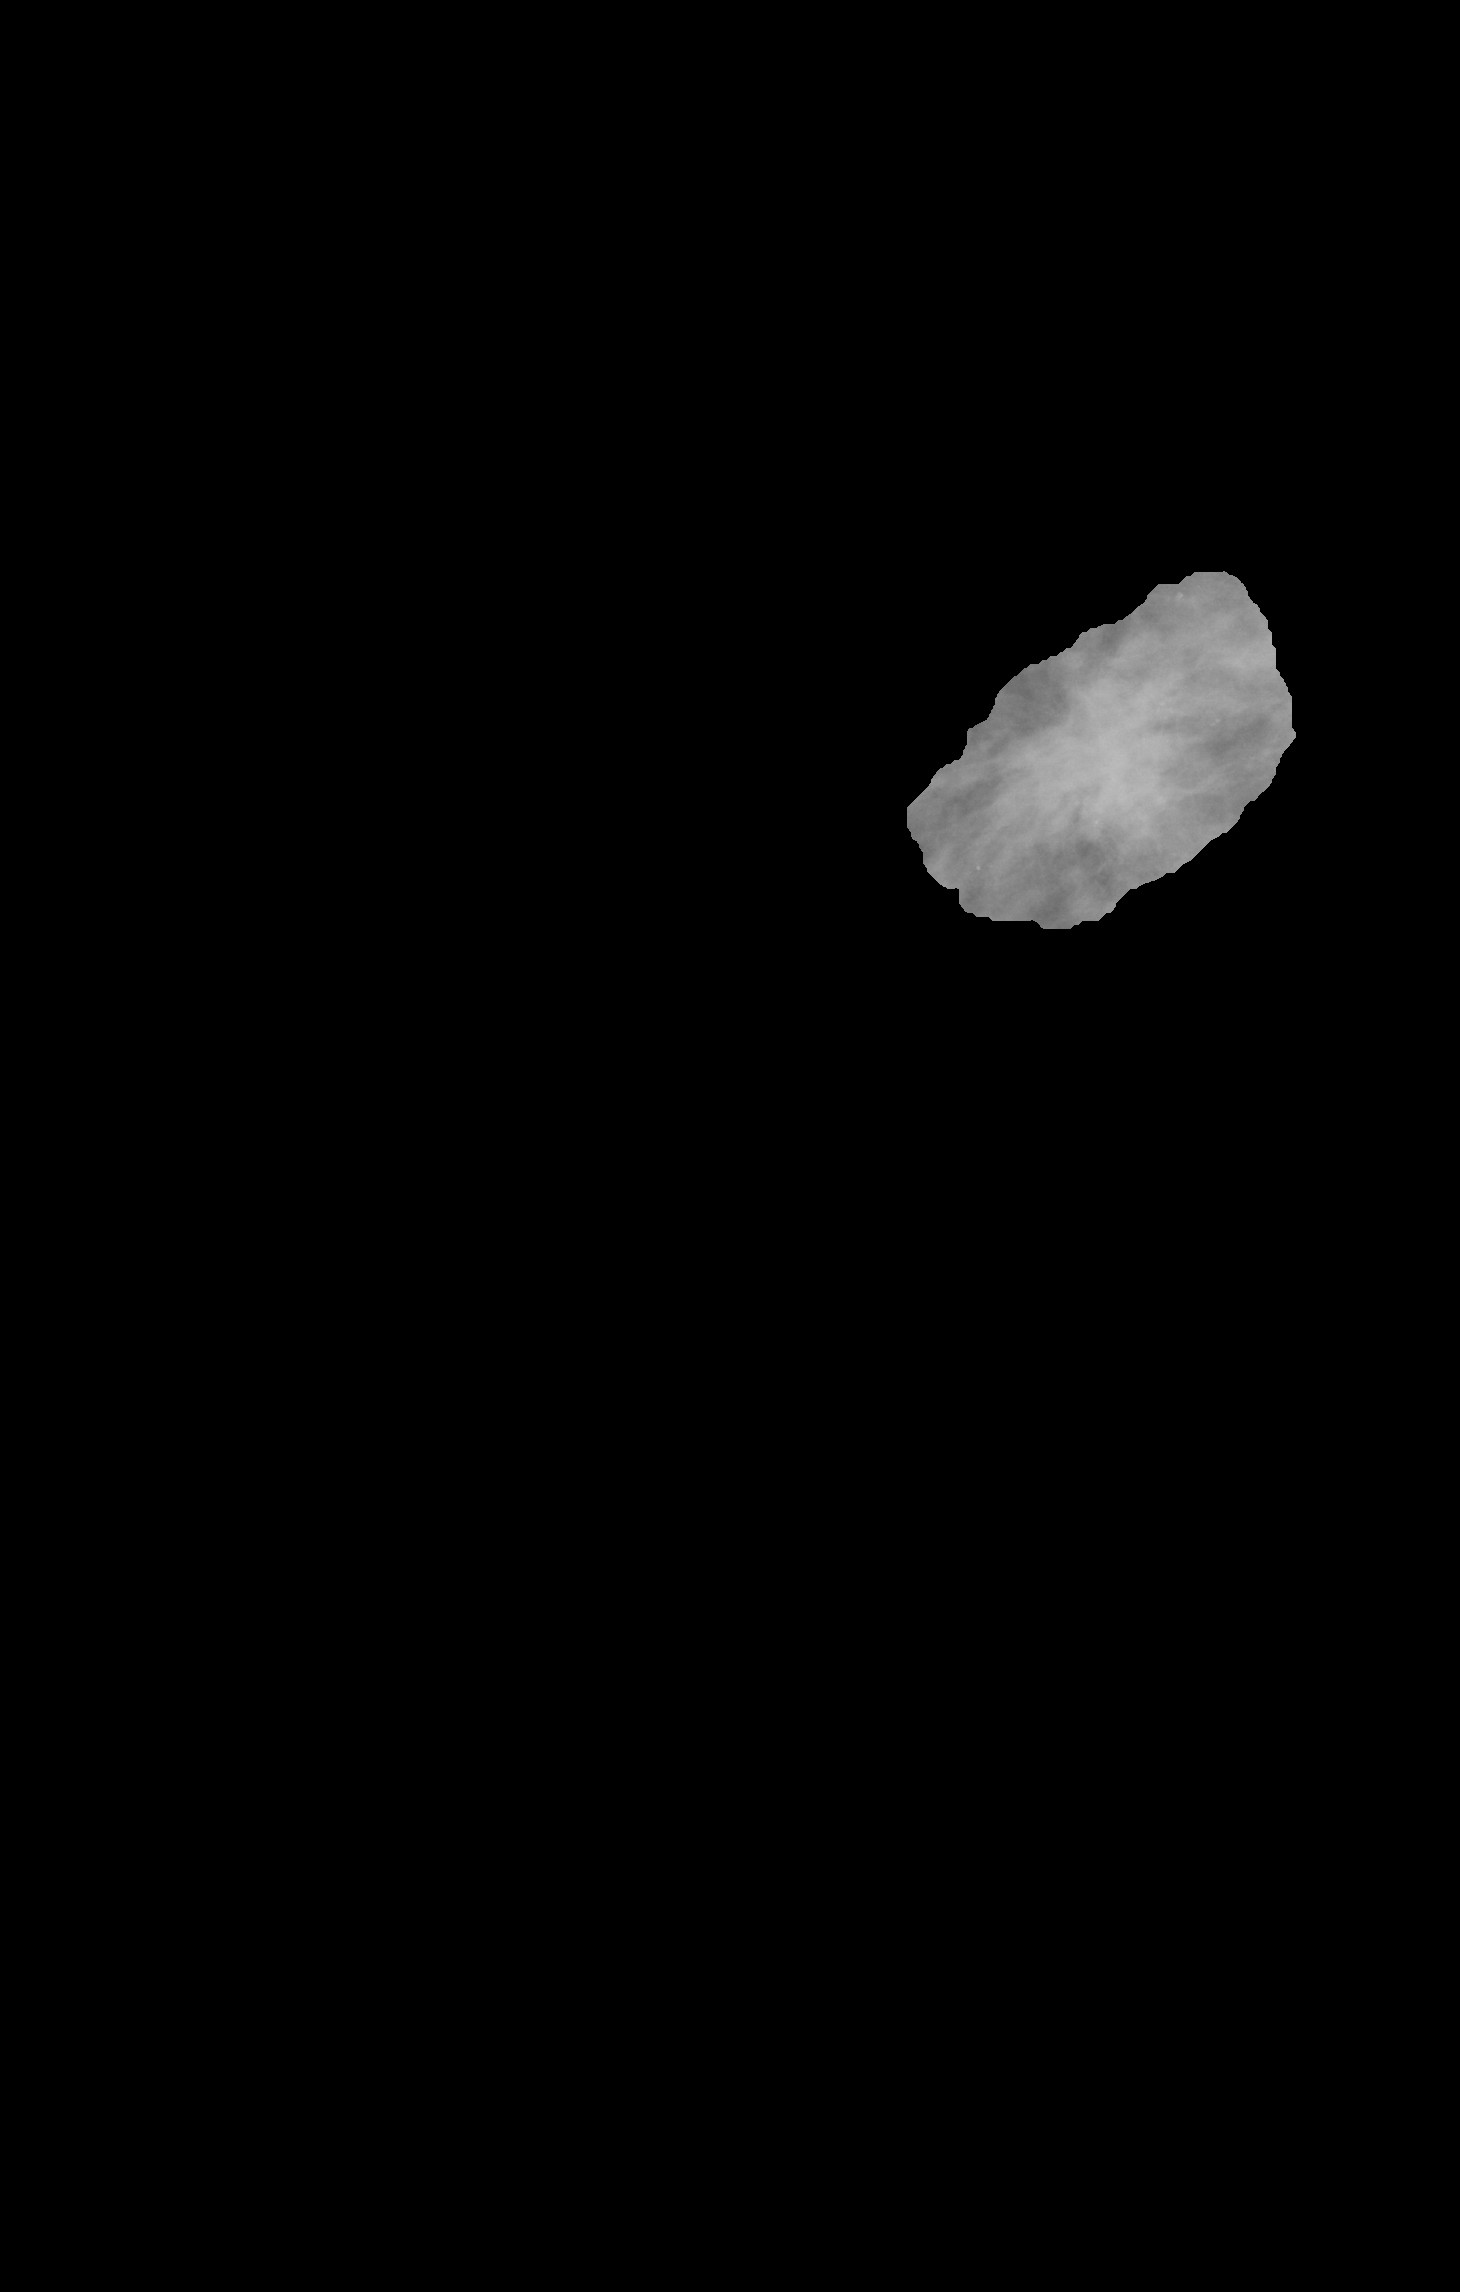
\includegraphics[width=4.5cm]{pics/Figures/result_img.jpg} }}%
		\caption{An image and the mask of the cancerous cell to isolate the cell from the rest of the image so the object detector would be able to learn the features of given cell with the isolation procedure beginning with the mask filled with ones, then overlapping the original image which contains the cancerous cell, the two images are then multiplied by each other making everything black except for whatever is inside the mask as seen in the \emph{Result Image}}
		\label{fig:img_cont}
	\end{figure}
	
	%There are three networks in the family of R-CNN object detector the original R-CNN \cite{RCNN}, Fast R-CNN \cite{Fast-RCNN} and Faster R-CNN \cite{Objdet} . In the original R-CNN network, selective search algorithm \cite{selective} is used to obtain region proposals. Afterwards, each proposal is fed into a \emph{CNN feature extractor} to obtain feature maps. In the last stage, the feature maps are input to \emph{support vector machines (SVM)} to obtain the class and bounding box of the proposed region. This approach is very time-consuming as it requires classifying a great amount of region proposals for each image. Therefore, \emph{Fast R-CNN} works on enhancing the inference speed. First features maps are produced by inputting the image into a \emph{CNN} feature extractor, then region proposals are created using the selective search algorithm. Afterwards, RoI pooling layer is used to reshape the proposal into a shape suitable for the \emph{FC} layers used for classification and bounding box regression.
	
	\subsubsection{Hierarchy Classification}\label{Hierarchy_Class}
	In \emph{Section~\ref{Classification}}, it has been explained that a classifier can classify between multiple classes, say there is three different classes $\bm{x}$ $\bm{y}$ and $\bm{z}$. These three classes have two classes which are quite similar, say that these similar classes are $\bm{x}$ and $\bm{y}$ sharing multiple features and are completely different from class $\bm{z}$ where they share no similar features. The classifier will be most likely to have a \textbf{larger error} when it comes to classifying between class $\bm{x}$ and $\bm{y}$, while it will be easier to classify class $\bm{z}$.\\[5mm]
	\begin{figure}[h]
		\centering
		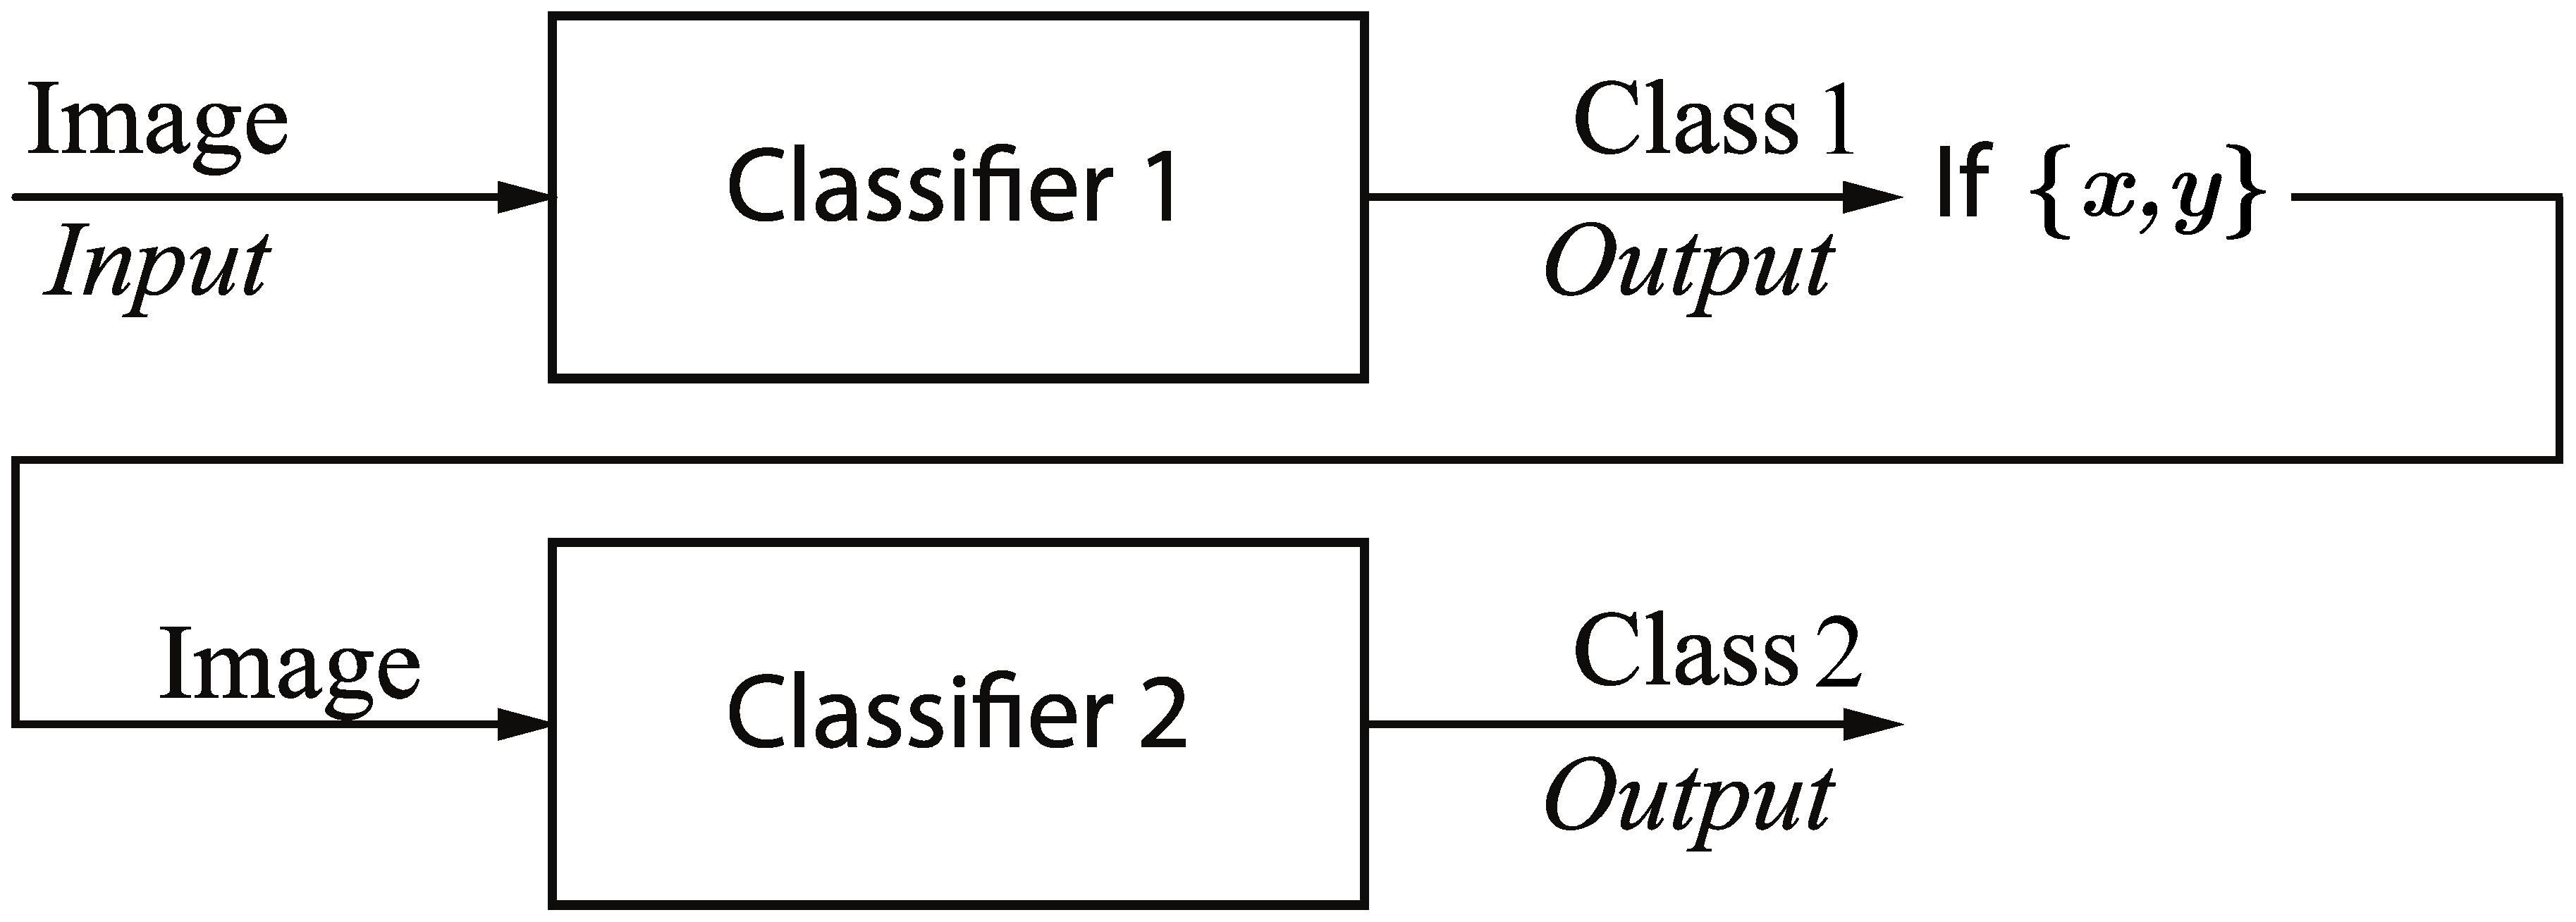
\includegraphics[width=0.7\textwidth]{pics/Figures/Hierarchical_Classifier_Block_Diagram.eps}
		\caption{\small{Hierarchical Classifier Diagram}}
		\label{fig:Hierarchical Classifier}
	\end{figure}
	This is where \textbf{Hierarchical Classification} comes into play, which could be graphically demonstrated in \emph{Figure \ref{fig:Hierarchical Classifier}}, as it will feature two separate classifiers, say one classifier to distinguish between two majorly different classes such as $\bm{\{x,y\}}$ and $\bm{z}$, this classifier will be denoted as \textbf{Classifier 1} which outputs \textbf{Class 1} that is a binary category on whether the input is classified as $\bm{z}$ or as $\bm{\{x,y\}}$. The reason that \textbf{Classifier 1} is set up is because it will be able to better distinguish between these two vastly different classes since it is easier to learn and distinguish their features, hence \textbf{Classifier 1} would be trained on the binary categorization, and if the output is classified as $\bm{\{x,y\}}$, then the same input will be taken to \textbf{Classifier 2}. \textbf{Classifier 2} is trained on discriminating between $\bm{x}$ and $\bm{y}$, and that is \textbf{Class 2}, which will give the classifier much better judgment over the two similar classes and have no third class interfere with the learning of the distinction between the two similar classes. This approach has been used in \cite{GJU} for x-ray image classification of patients with Pneumonia, Covid-19 \emph{(Unhealthy)} or Neither \emph{(Healthy)}. This Hierarchy can be seen in \emph{Figure~\ref{fig:GJU}}.
	\begin{figure}[h]
		\centering
		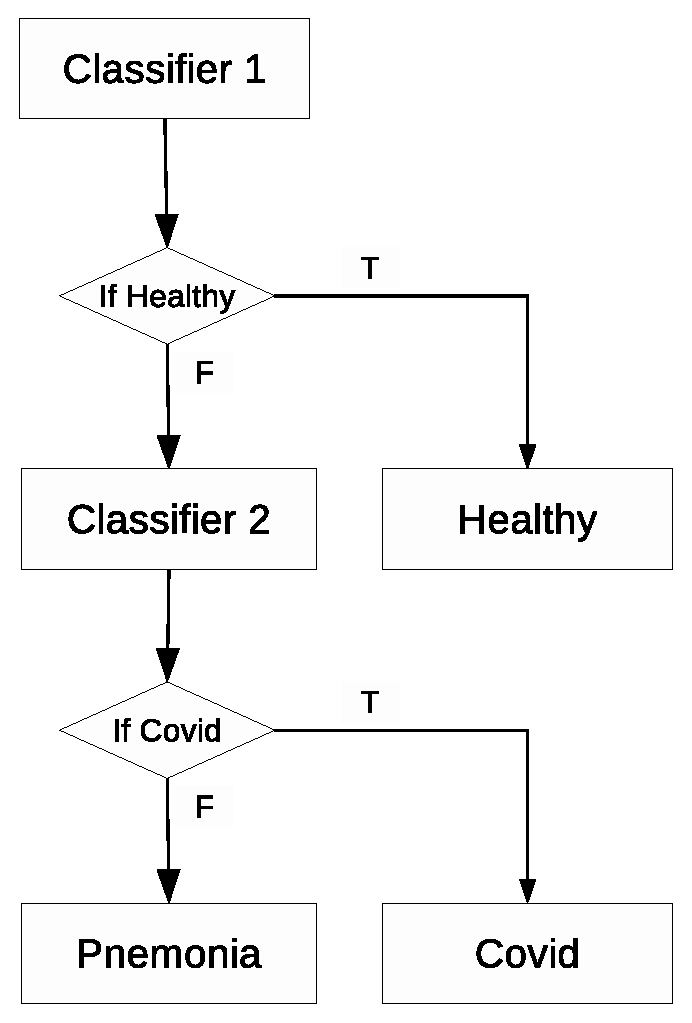
\includegraphics[width=0.5\textwidth]{pics/Figures/GJU_H.eps}
		\caption{\small{Hierarchical Classifier Flowchart}}
		\label{fig:GJU}
	\end{figure}
	
	\subsubsection{Multi-Stage Object Detector}\label{Meth}
	\emph{Single-Stage} object detectors work with having the classification process happen at the end of the detector since that is the quicker method, hence the name given to it is the \emph{"Single-Stage"}. However, in \emph{Two-Stage} object detectors, the object detector works on a single model and then if a detector detects an object, it is passed to another model and that is the second stage which is a classifier, hence the name \emph{"Two-Stage"} object detector is given and is also called the \textbf{Multi-Stage Object Detector (MSOD)}, this can be clearly seen on how insignificant it is in regards to inference speed in comparison to the Single-Stage object detector.\\[5mm]
	\emph{Figure \ref{fig:Multi-Stage Obj Detector}} shows the work-flow of a \emph{MSOD}.\\[5mm]
	\begin{figure}[h]
		\centering
		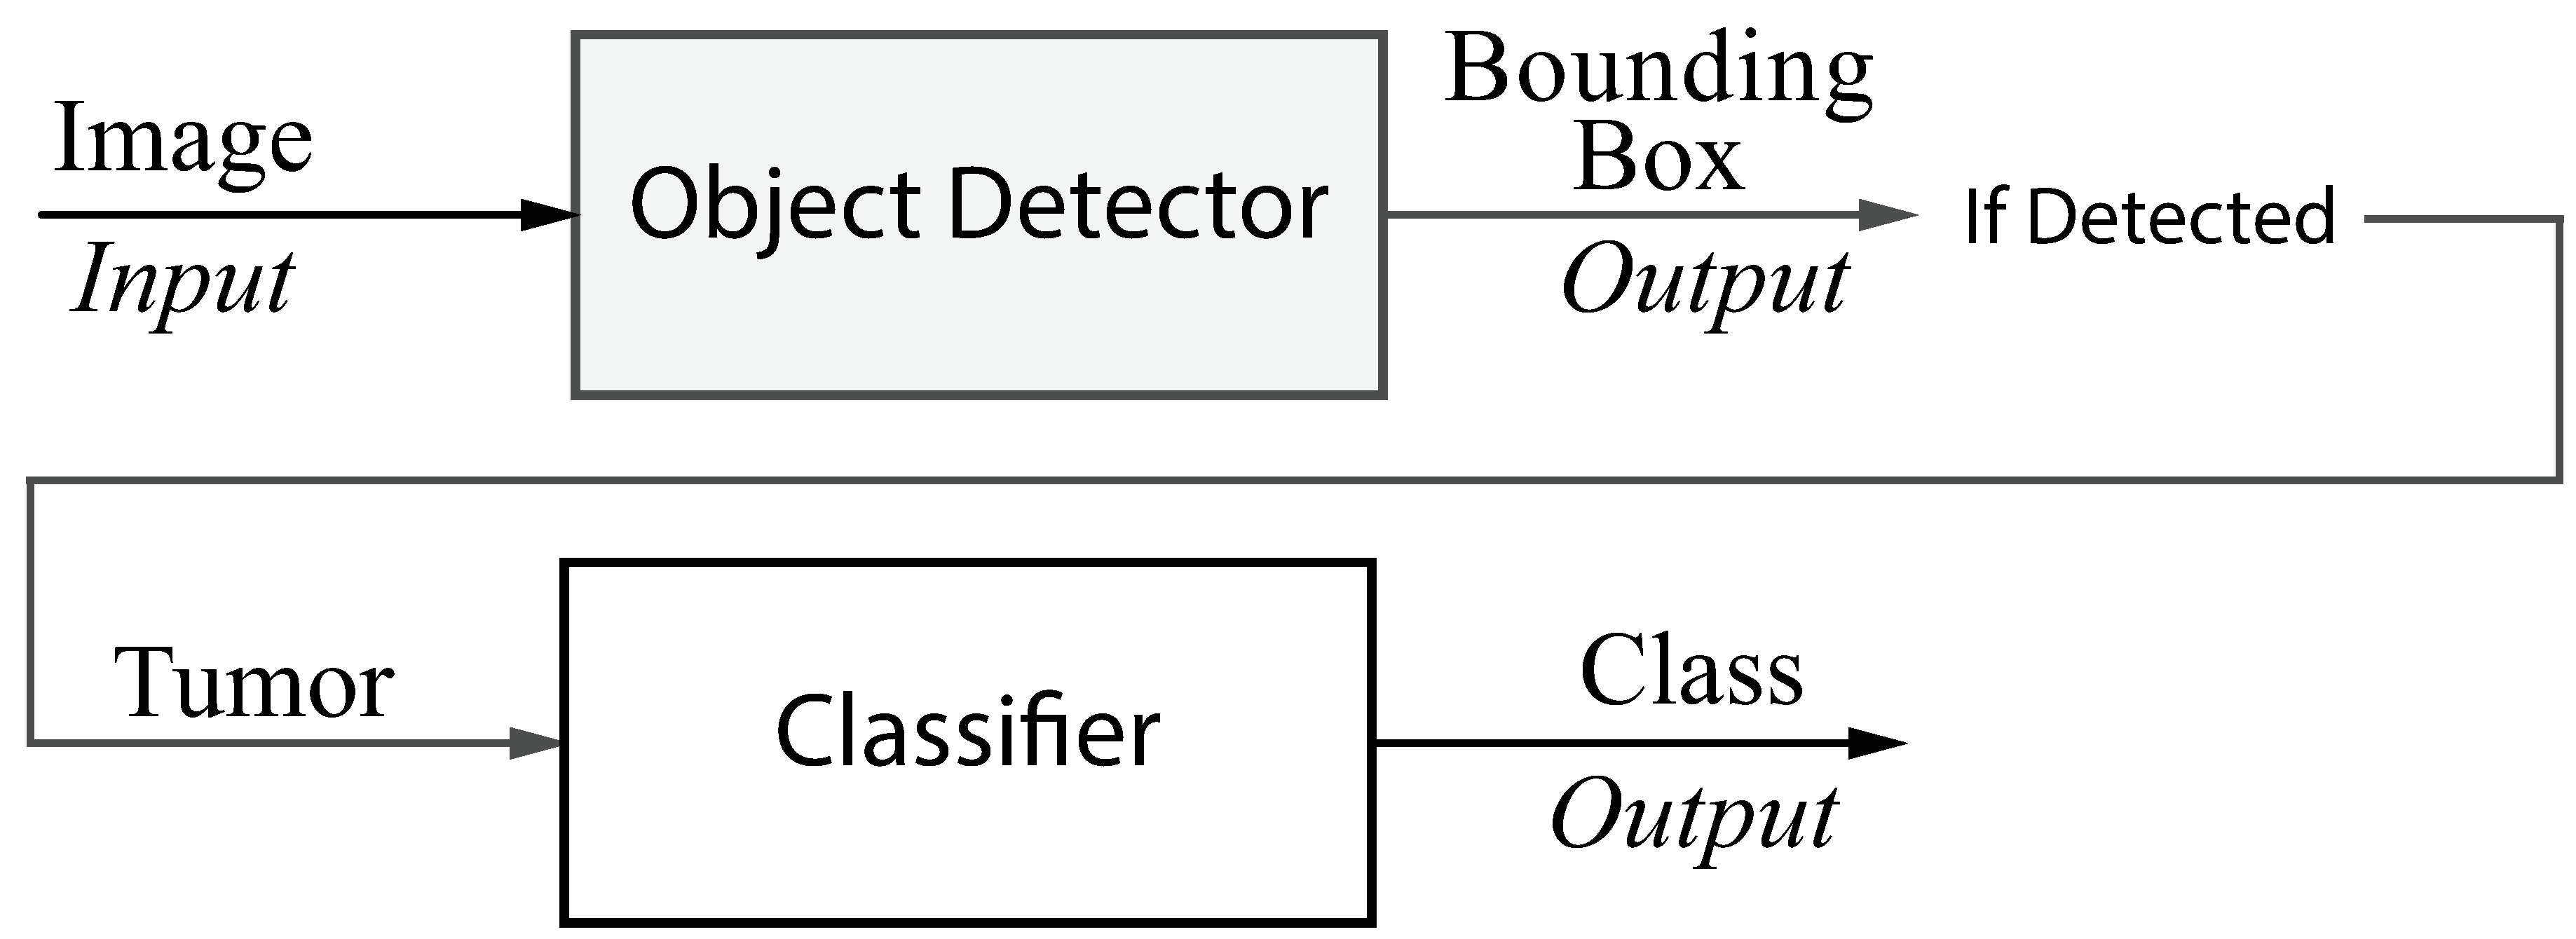
\includegraphics[width=0.7\textwidth]{pics/Figures/Hierarchical_Obj_Det_Block_Diagram.eps}
		\caption{\small{Multi-Stage Object Detection Diagram}}
		\label{fig:Multi-Stage Obj Detector}
	\end{figure}
	The importance of using a \emph{MSOD} rather than a Single-Stage object detector is mainly due to the higher accuracy that will be acquired by the model since the object detector is separated from the classifier and each carries out a different task, the detector focusing on the features of the tumor and detecting the tumor, no matter which \emph{Class} said tumor is given to, while the classifier would receive an image solely of the tumor rather than the whole raw image, as would the second classifier from the \emph{Hierarchical Classifiers} in \emph{Section~\ref{Hierarchy_Class}} receive and that being the whole image. \emph{Figure~\ref{fig:cropped}} shows the cropped image of the tumor entering the classifier in the \emph{MSOD} model as a product from \emph{Figure~\ref{fig:img_cont}}.
	\begin{figure}[h]
		\centering
		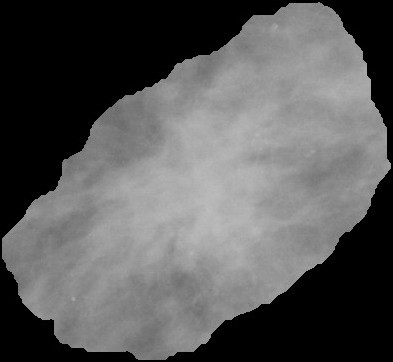
\includegraphics[width=0.5\textwidth]{pics/Figures/cropped.jpg}
		\caption{\small{Cropped input for \emph{MSOD} Classifier}}
		\label{fig:cropped}
	\end{figure}
	Having a cropped image of the tumor as an input for a classifier would help focus all the attention on the features of the two different kinds of tumors, thus improving the learned features, while correspondingly reducing the amount of learning parameters as the input size would be smaller hence reducing computational effort and time. 
	
	\newpage
	\section{Design}
	This section will discuss the appropriate approach which was taken for performing the detection and the differentiation of the tumor cells found in the breast.
	
	
	\subsection{Methodology}
	Initial approach to starting is by gathering the required dataset, this was possible due to an open-source dataset which was found on \href{https://www.kaggle.com/}{Kaggle}, this website hosts multiple competitions in Machine Learning and Data Science domains, apart from competitions, the website also gathers open-source data. With this valuable resource acquired, the dataset under the name of \emph{Mini-DDSM} (Digital Database for Screening Mammography) \cite{Dataset} was used due to the accurate labeling made by professionals and the high quality and great quantity of images. Further discussion about the dataset will be found in \emph{Section~\ref{Data}}.
	
	\subsubsection{Virtual Environment}
	To begin the process of writing the script for implementing the project there must be a standard library version use across the directory which contains the code-base, and that is by setting up a virtual environment \emph{locally} where the versions of the libraries could be isolated to eliminate version conflicts and imply a stable version dependency. \textbf{\textit{Anaconda}} already allows this functionality where multiple virtual environments could be set up on a single local machine \cite{anaconda}. With Anaconda's help, a virtual environment could be set up to help download and install all the required libraries and packages to run the code. The most prominent libraries and packages where \textbf{\textit{Tensorflow}} \cite{tensorflow2015-whitepaper}, \textbf{\textit{Keras}} \cite{chollet2015keras} and \textbf{\textit{NumPy}} \cite{harris2020array}, along many other packages which were used that could be found in \emph{Appendix~\ref{libraries}}.
	
	\subsubsection{Google Colaboratory}
	Apart from local work, which was not computationally intensive, there were some sections of the project which were extremely computationally demanding and for these components, the cloud computing was helpful as there was no need to execute the code locally but rather using the cloud platform known as \emph{\href{https://research.google.com/colaboratory/}{Google Colab}} also known as \emph{Colab}. In addition, this platform grants limited use of a GPU which was heavily utilized in the process of this project.\\
	Another positive aspect of using Colab is that all the required libraries are \textit{pre-installed} on their servers and are used quickly without the need to install them.
	
	
	\subsection{Dataset}\label{Data}
	Choosing a dataset for this problem is crucial to many stages, first and foremost is the \emph{quality of the data}. Does the data clearly portray the goal that should be acquired? Secondly is the \emph{quantity of the dataset}, just like the quality, quantity is as important. \textbf{Neural Networks} require a lot of data, but the quantity mainly depends on the following:
	\begin{itemize}
		\item features that must be extracted from the data
		\item type of Neural Network
		\item data quality
		\item the desired goal
	\end{itemize}
	With that being said, the data is a vital part of this project, and to be able to achieve high accuracy and precision of detecting the cancerous cells, it is a must to obtain high grade dataset. 
	The most common age for the diagnosis of breast cancer is \emph{over 50} years of age. This has been conducted by the National Cancer Institute that the median age of breast cancer patients is between the age of \emph{55} to \emph{64} \cite{CDC}. 
	\\[5mm]
	\subsubsection{Data collection and statistics}\label{Data_collection}
	In this graduation project, the procedure for \emph{data collection} was straight-forward as there is an already published dataset \cite{Dataset} with the purpose of research that was used in this graduation project. There is quite astonishing remarks regarding the dataset as it holds data for \textbf{1.952} patients with \textbf{4 images per patient}, two views per breast, which sets the total number of data to \textbf{7.808 images} in possession for processing, analyzing and configuring.\\[5mm]
	Some constraints and observations were met regarding the labeling of the data where a patient is diagnosed as \emph{Cancer} or \emph{Benign} based on the presence of the tumor in at least one of their breast. While that could be true for the case of the patient, however, it is false labeling when it comes to the methodology this graduation project documentation follows as a breast which does not contain any tumor cannot be labeled as not \emph{Normal}, this case could be seen in \emph{Table~\ref{data_label}}.
	\begin{center}
		% Please add the following required packages to your document preamble:
		% \usepackage[table,xcdraw]{xcolor}
		% If you use beamer only pass "xcolor=table" option, i.e. \documentclass[xcolor=table]{beamer}
		\begin{table}[]
			\caption{A preview for the labeling of the dataset}
			\begin{tabular}{llllll}
				\hline
				\label{data_label}
				\cellcolor[HTML]{222A35}{\color[HTML]{E7E6E6} fileName} & \cellcolor[HTML]{333F50}{\color[HTML]{E7E6E6} View} & \cellcolor[HTML]{8497B0}{\color[HTML]{E7E6E6} Side} & \cellcolor[HTML]{8994A1}{\color[HTML]{E7E6E6} Status} & \cellcolor[HTML]{8A9A8F}{\color[HTML]{E7E6E6} Age} & \cellcolor[HTML]{717F74}{\color[HTML]{E7E6E6} Tumour\_Contour} \\ \hline
				\rowcolor[HTML]{D0CECE} 
				C\_0236\_1.LEFT\_CC.png                                 & CC                                                  & LEFT                                                & Benign                                                & 67                                                 & -                                                              \\
				\rowcolor[HTML]{D0CECE} 
				C\_0236\_1.LEFT\_MLO.png                                & MLO                                                 & LEFT                                                & Benign                                                & 67                                                 & -                                                              \\
				\rowcolor[HTML]{D0CECE} 
				C\_0236\_1.RIGHT\_CC.png                                & CC                                                  & RIGHT                                               & Benign                                                & 67                                                 & RIGHT\_CC\_Mask.png                                            \\
				\rowcolor[HTML]{D0CECE} 
				C\_0236\_1.RIGHT\_MLO.png                               & MLO                                                 & RIGHT                                               & Benign                                                & 67                                                 & RIGHT\_MLO\_Mask.png                                           \\
				\rowcolor[HTML]{F2F2F2} 
				B\_3008\_1.LEFT\_CC.png                                 & CC                                                  & LEFT                                                & Cancer                                                & 53                                                 & -                                                              \\
				\rowcolor[HTML]{F2F2F2} 
				B\_3008\_1.LEFT\_MLO.png                                & MLO                                                 & LEFT                                                & Cancer                                                & 53                                                 & -                                                              \\
				\rowcolor[HTML]{F2F2F2} 
				B\_3008\_1.RIGHT\_CC.png                                & CC                                                  & RIGHT                                               & Cancer                                                & 53                                                 & RIGHT\_CC\_Mask.png                                            \\
				\rowcolor[HTML]{F2F2F2} 
				B\_3008\_1.RIGHT\_MLO.png                               & MLO                                                 & RIGHT                                               & Cancer                                                & 53                                                 & RIGHT\_MLO\_Mask.png                                           \\
				\rowcolor[HTML]{D0CECE} 
				A\_0218\_1.LEFT\_CC.png                                 & CC                                                  & LEFT                                                & Normal                                                & 59                                                 & -                                                              \\
				\rowcolor[HTML]{D0CECE} 
				A\_0218\_1.LEFT\_MLO.png                                & MLO                                                 & LEFT                                                & Normal                                                & 59                                                 & -                                                              \\
				\rowcolor[HTML]{D0CECE} 
				A\_0218\_1.RIGHT\_CC.png                                & CC                                                  & RIGHT                                               & Normal                                                & 59                                                 & -                                                              \\
				\rowcolor[HTML]{D0CECE} 
				A\_0218\_1.RIGHT\_MLO.png                               & MLO                                                 & RIGHT                                               & Normal                                                & 59                                                 & -                                                              \\ \hline
			\end{tabular}
		\end{table}
	\end{center}
	Hence, all the patients that were diagnosed with a tumor in a single breast would be automatically diagnosed the same status in the other breast even though it is clear that the second breast does not contain any tumor as seen in \emph{Table~\ref{data_label}}, patient \emph{No. 0236} where only their right breast contains \emph{Benign} cells but their left breast did not contain any tumors. Taking pictures individually with the patient's label is a wrong approach to training an \emph{Image Classifier} as it will \emph{"confuse"} the model and stray it off and the model will start learning the wrong features.\\[5mm]
	Some other special cases where found such as a patient containing multiple tumors in one breast, containing tumors in both their breasts and in very rare occasions only having the tumor detected in one view rather as in both views.\\[5mm]
	These ordinary and extra ordinary cases will be taken care off so that there will not be any case of \textbf{miss-labeling} of any data.\\[5mm]
	Some statistics regarding patients is shown in \emph{Figure~\ref{fig:Age_Dist}} and \emph{Figure~\ref{fig:Avg_Age}}.
	
	\begin{figure}[h]
		\centering
		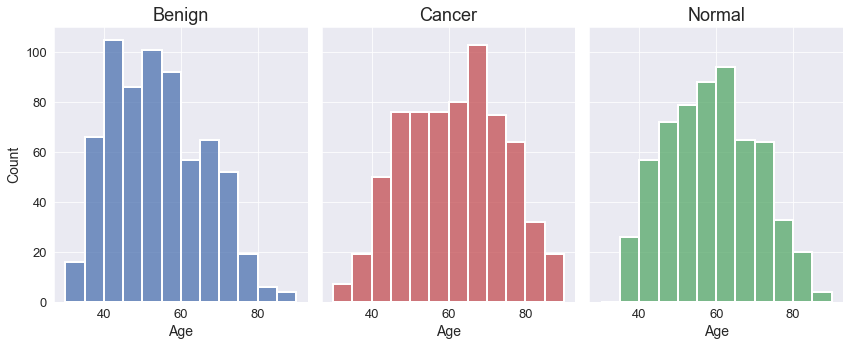
\includegraphics[width=1\textwidth]{pics/Figures/Age_Dist.png}
		\caption{\small{Age Distribution}}
		\label{fig:Age_Dist}
	\end{figure}
	\begin{figure}[h]
		\centering
		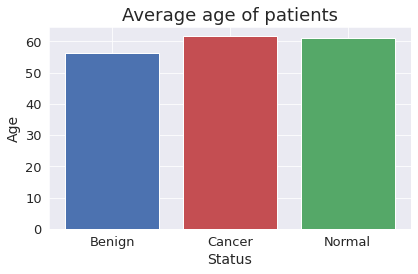
\includegraphics[width=0.5\textwidth]{pics/Figures/Avg_Age.png}
		\caption{\small{Average Age}}
		\label{fig:Avg_Age}
	\end{figure}
	\newpage	
	\subsubsection{Data imbalance}\label{imbalance}
	After performing the method described in \emph{Section~\ref{Data_collection}}, the dataset will be thrown into an imbalanced state where the amount of Normal (Tumor-less) images are severely outnumbering the two other cases, this can be seen in \emph{Figure~\ref{fig:imbalance}}.
	\begin{figure}[h]
		\centering
		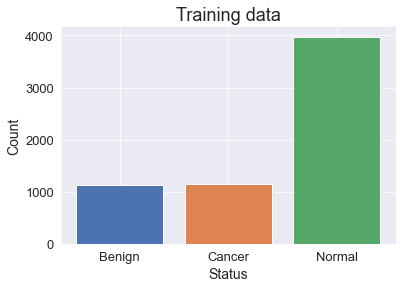
\includegraphics[width=0.5\textwidth]{pics/Figures/Train_imbalance.png}
		\caption{\small{Visualization of imbalanced dataset}}
		\label{fig:imbalance}
	\end{figure}
	
	As seen in the above figure, the dataset is 1:1:4 where the normal cases are \textbf{x4} the amount of the Benign and Cancer cases.
	to counter this we simply store 1 Normal case for every 4 cases that are encountered. The Listing below explains the function that was used to counter the imbalance set.

	After implementing this snippet into the \textbf{DataLoader}, the dataset imbalance was resolved, as could be seen in the figure below.
	\begin{figure}[h]
		\centering
		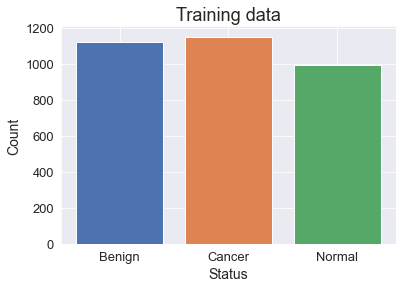
\includegraphics[width=0.5\textwidth]{pics/Figures/Train_balance.png}
		\caption{\small{Visualization of resolved imbalance}}
		\label{fig:balance}
	\end{figure}
	On another note, for the \textbf{Validation Data}, this imbalance will not affect the results in any way.
	
	\subsection{Data Pipeline}
	The process of handling the dataset is crucial when it comes to Deep Learning or any sort of AI projects as a \emph{Data-Loader} could quite easily act as a bottle-neck in a completed project.\\
	Creating a Data-Loader requires the use of Object Oriented Programming which was possible to perform in \emph{Python} programming language. Since the main sub-library \textbf{\textit{Keras}} is responsible for the architecture and the build of the \emph{Neural Networks}, Keras also provides a Data-Loader class, named \textbf{\textit{Sequence}}, which was utilized by inheriting it into the custom made Data-Loader that is implemented in this graduation project.\\
	The objective of a Data-Loader is to load, preprocess and feed the data, by batches, into the \textbf{\textit{Neural Network Model}}, which could also be referred to as \emph{Model}. So in this subsection, the three main stages of loading the data into the model will be discussed in the following order.
	\begin{itemize}
		\item Data Loading
		\item Data Preprocessing
		\item Batch feeding
	\end{itemize}
	
	It was helpful to locate the path of each image from an included \emph{Comma Separated Values} (CSV) file in the \emph{Mini-DDSM} dataset which was collected for this project. This CSV file contained all the labeling and all the paths of the images, as seen in \emph{Table~\ref{data_label}}. The process of the data pipeline will be as illustrated in \emph{Figure~\ref{fig:pipeline}}.
	\begin{figure}[h]
		\centering
		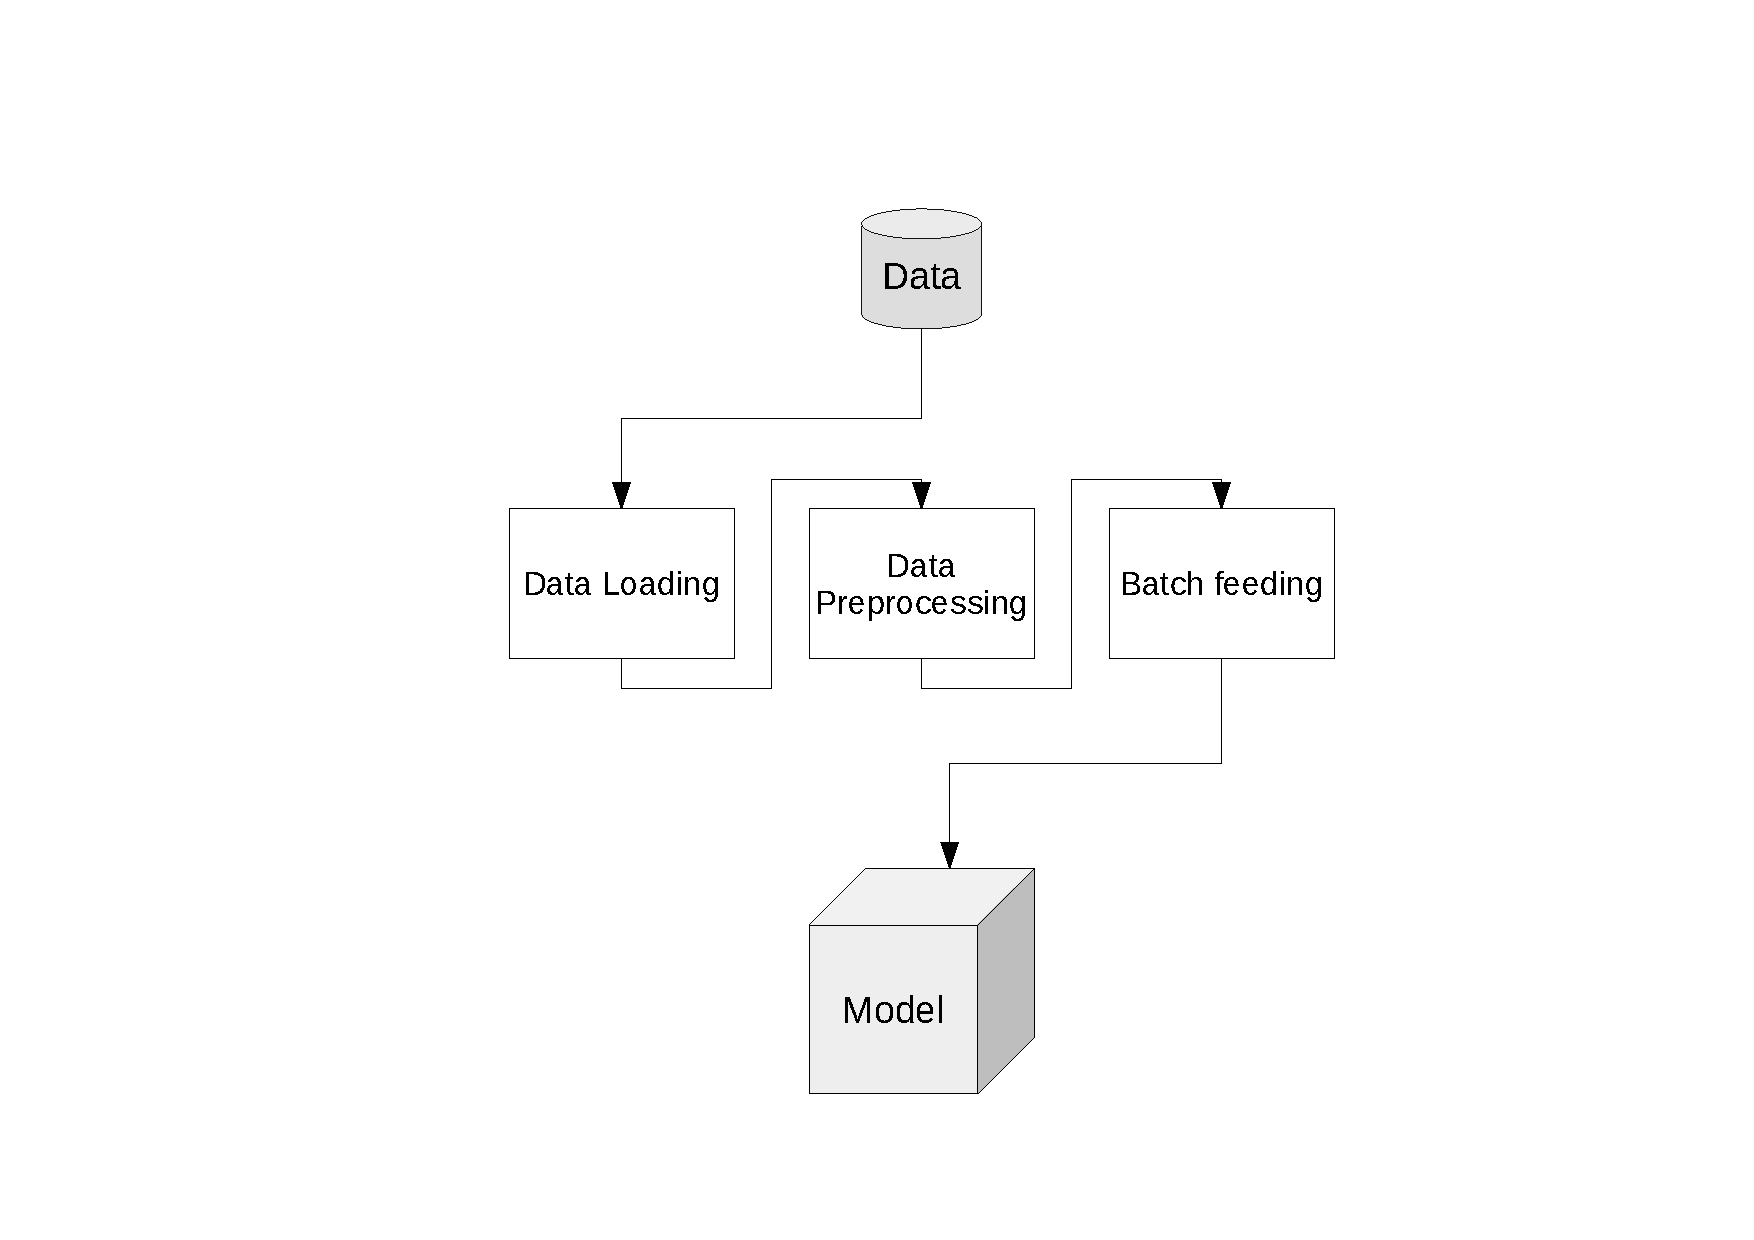
\includegraphics[width=1\textwidth]{pics/Figures/Data_pipeline.pdf}
		\caption{\small{Illustration of data pipeline}}
		\label{fig:pipeline}
	\end{figure}
	
	\subsubsection{Data Loading}
	The data loading function would start off by collecting all of the paths from the CSV file and convert them into a \emph{list of paths}, this was crucial to have the ability to iterate through the paths without having the need to refer back to the CSV file and would additionally be much more easier to manipulate, for example, shuffle and provide custom conditions to the list.\\
	Here there were 3 sets of empty lists created with labels of each corresponding case \emph{(Normal, Cancer or Benign)}. As the iteration flows through the CSV file, there would be a custom condition set to collect the Cancer labeled images' path into the `Cancer` labeled list, the Benign images' path into the `Benign` labeled list and the Normal images' path into the `Normal` labeled list. But for each 4 Normal images we would append only 1 image into the list for the imbalance case as seen in \emph{Section~\ref{imbalance}}. This allows for separation in each class so there will not be any mislabeling happening which could confuse the \emph{Model} while training or provide false results during evaluation.\\
	The custom Data-Loader has been modified from the \emph{Sequence} inheritance by performing \emph{memory-extensive} loading, this is desperately needed as the local machine which was used for the creation of this project had limited physical memory and upon loading the data, the machine was subjected to \emph{run out of memory}, this was countered by loading the data in batches, which will be discussed in \emph{Section~\ref{preproc}}, this also includes preprocessing in batches which will be discussed in \emph{Section~\ref{batching}}.
	 \begin{figure}[h]
	 	\centering
	 	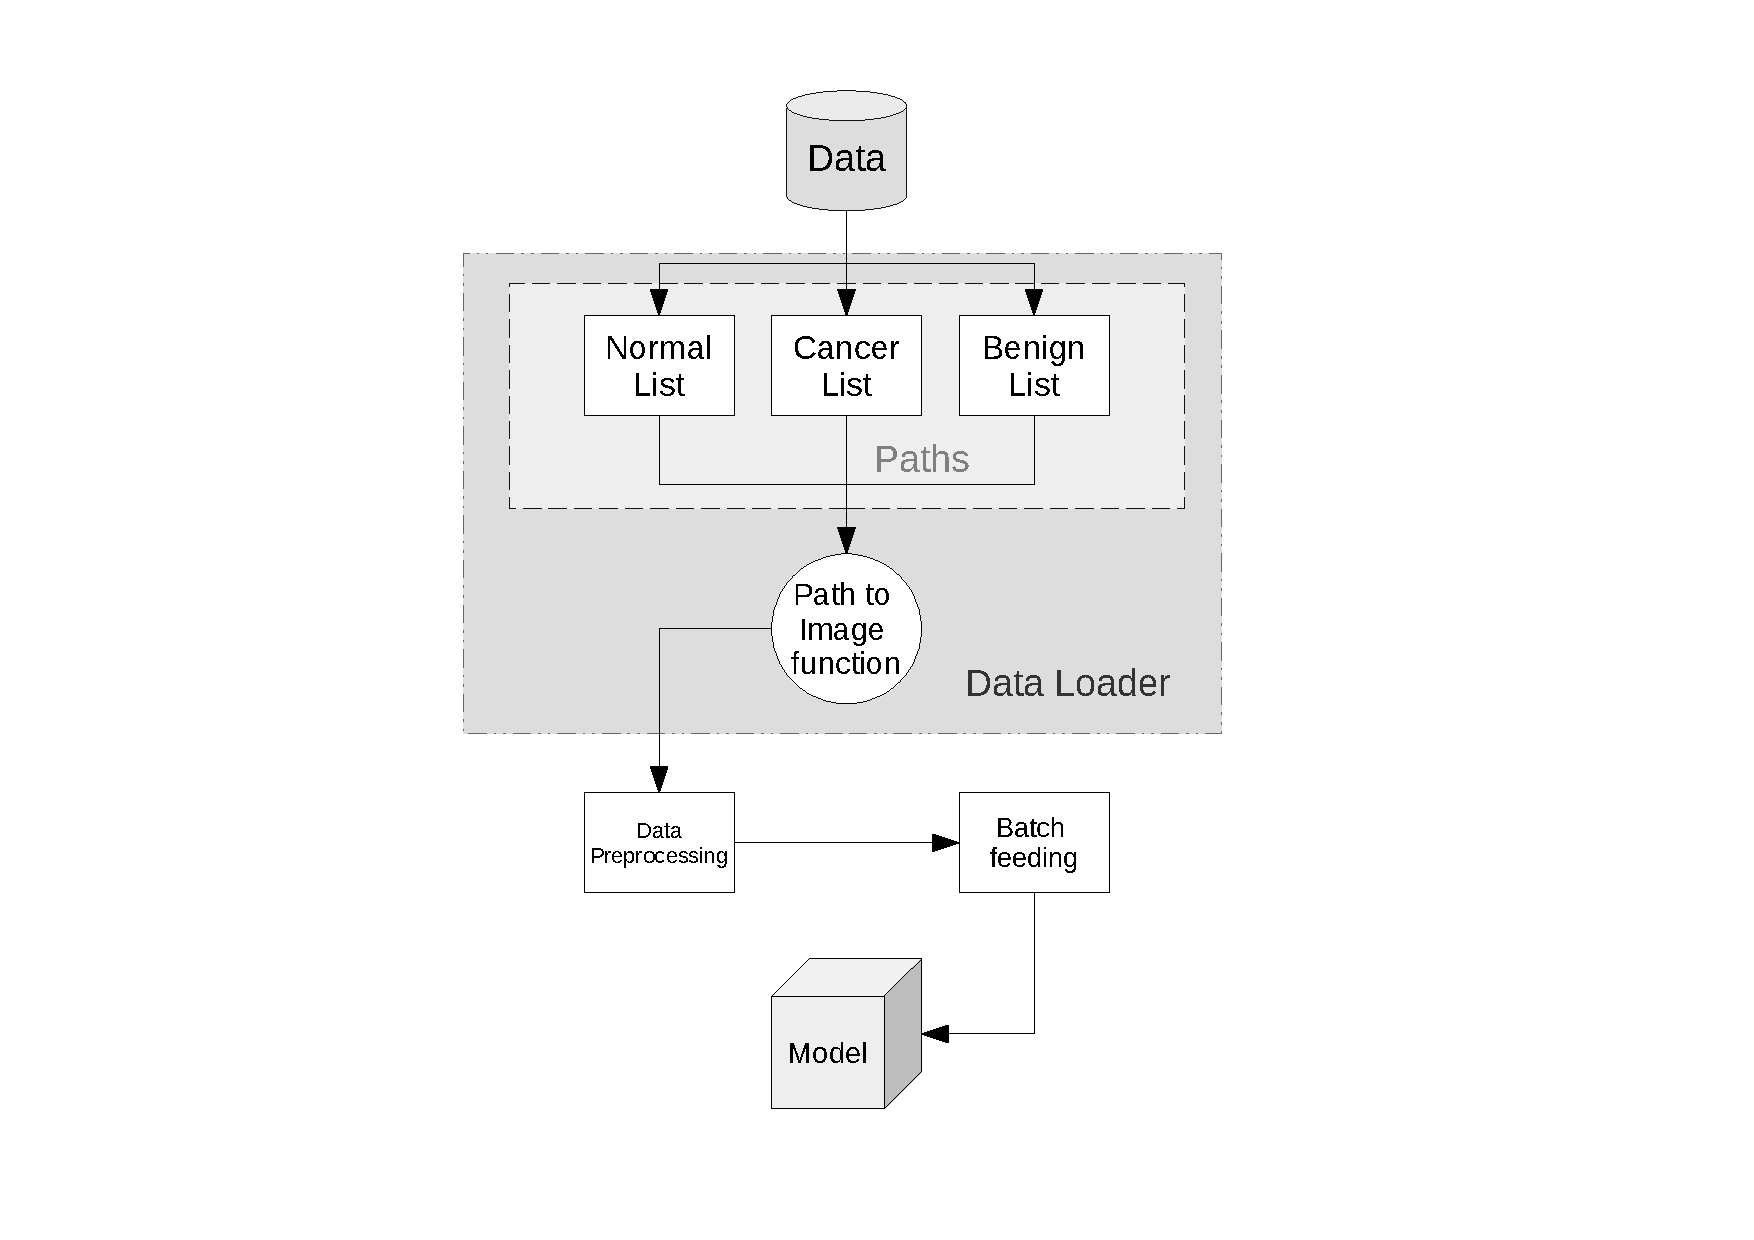
\includegraphics[width=1\textwidth]{pics/Figures/Data_loader.pdf}
	 	\caption{\small{Illustration of data loader}}
	 	\label{fig:Data_loader}
	 \end{figure}
	
	\subsubsection{Data preprocessing}\label{preproc}
	After loading the images from the paths, the next step into readying the dataset for the \emph{Model} would be by preprocessing the images. This will achieve unification of image sizes, as the size of the \emph{Model} input shall remain the same, and the process of augmenting the training data to reduce over-fitting of the \emph{Model}.\\
	Even though the open-source \emph{Mini-DDSM} dataset lacked almost nothing, it had one flaw and that was the different sizes that each image had, with such varying sizes, this imposed an issue for the \emph{Model} as the input size, or shape, of the first layer shall always remain the same size, hence the preprocessing of the whole dataset shall take place. Since the \emph{aspect-ratio} of the images also vary this means that having a constant width or height of an image will be deemed impossible since the area of the image will never equal to the rest of the images, this is why resizing alone will not be effective but shall be accompanied with a zero padding to the remaining gaps, whether being along the top and bottom or left and right sides of the images.\\
	The mean of the widths and the mean of the heights of the images were calculated and that was the chosen desired width and length of the image sizes which will be input into the \emph{Model}.\\
	
	
	\subsubsection{Batch Feeding}\label{batching}
	This method of intensely reducing memory usage was performed by utilizing the \emph{list of paths} and with the functionalities of the inherited class \emph{Sequence}, that was by calling a \emph{fetching function}, known as \emph{\textbf{\_\_getitem\_\_}}, the Model was able to acquire a preprocessed batch which would be ready for training.
	
	\subsection{Image Classifier}
	The first approach to creating the MSOD model is to create the initial classifier which will be a broader approach to detecting whether the patient is diagnosed with \emph{Cancer}, \emph{Benign} or has no Tumor \emph{(Normal)}. Unfortunately, during training, the whole image is passed which could be seen in \emph{Figure~\ref{fig:img_cont} (a)}, and that contains many unwanted features that will reduce the performance of the trained model.
	In the figure below, the confusion matrix is shown for the first stage image classifier which was discussed in \emph{Section~\ref{Classification}}.
	\begin{figure}[h]
		\centering
		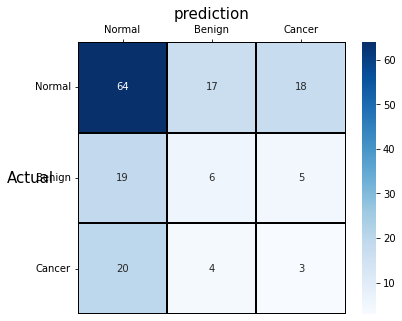
\includegraphics[width=0.6\textwidth]{pics/Figures/1st_stage_conf_matrix.png}
		\caption{\small{Confusion matrix of the first stage Classifier}}
		\label{fig:conf-mat-first}
	\end{figure}
	Some quick analysis from this Confusion Matrix is that the model has learned to classify the Normal vs Tumor in an almost efficient way. But given that the labels are not \emph{`Normal`, `Tumor`} but rather \emph{`Normal`, `Benign`, `Cancer`}, the model had a hard time differentiating between the two tumor classes. Which is why the \textbf{Hierarchy Classifier}, which was discussed in \emph{Section~\ref{Hierarchy_Class}}, will achieve better results given that the first stage classifier will predict the two classes \emph{`Normal`, `Tumor`} and the second classifier will have the task of differentiating between \emph{`Benign`, `Cancer`}.
	
	\subsection{Hierarchy Classifier}
	
	code for running Hierarchy Classifier
	
	\begin{lstlisting}[language=Python, caption=Backbone layer unlocking function, label=unlock]
		def unfix_layers_Backbone_weights(self, Nlayer=3):
		"""To unfix the backbone weights
		
		Args:
		Nlayer (int, optional): the amount of layers to unfix from the end. Defaults to 3.
		"""
		for i, _ in enumerate(self.model.layers[-5 - Nlayer:]):
		self.model.layers[i].trainable = True
	\end{lstlisting}

	\subsection{Transfer Learning}
	In transfer learning, it is crucial to keep the \emph{pre-trained weights} intact, at least most of them from the upmost layers, because they are the most important weights when it comes to feature extraction. 
	
	
	
	This allows the last 3 layers of the backbone to unlock and be able to \emph{fine-tune} to our own custom dataset.
	
	\subsection{Training}
	Some text about training 
	
	Some text about training classifier with backbone
	
	

	\newpage
	
	\section{Results and Discussions}
	 \subsection{Single Classifier}
	 With transfer learning using the \textbf{Efficient Net b-0}, the accuracy of 46.8\% was achieved.\\
	
	\section{Conclusion}
	In conclusion, in this graduation project, the main objective will be to undergo several cases which were listed in \emph{Section~\ref{CV}} and end the graduation project with the chosen method which is a \emph{Multi-Stage Object Detector (Two-Stage object detector)}, this focuses on bridging the gap in paper \cite{one_shot} where the chosen approach was a \emph{Single-Stage object detector}. In theory, this should improve the results since it is known that Two-Stage object detection prioritizes accuracy over inference speed while Single-Stage object detectors rather sacrifice accuracy for inference speed (as used in \cite{one_shot}). 
	\subsection{Future work}
	For MSOD 
	\newpage

	\bibliographystyle{IEEEtran}
	\bibliography{IEEEabrv,myrefs}
	
	
\end{document}

\newpage
\setstretch{1}  %reduce bibliography line spacing
\end{document}